%Dokumentinformationen
\newcommand{\titleinfo}{Complexe Zahlen, Fourierreihen - Formelsammlung}
\newcommand{\authorinfo}{D. Koeppel, L. Leuenberger}
\newcommand{\versioninfo}{$Revision: 2.2 $ - powered by \LaTeX}

% standard header
%%Schriftgr�sse, Layout, Papierformat, Art des Dokumentes
\documentclass[10pt,twoside,a4paper,fleqn]{article}
%Einstellungen der Seitenr�nder
\usepackage[left=1cm,right=1cm,top=1cm,bottom=1cm,includeheadfoot]{geometry}
% Sprache, Zeichensatz, packages
\usepackage[utf8]{inputenc}
\usepackage[ngerman]{babel,varioref}
\usepackage{amssymb,amsmath,fancybox,graphicx,color,lastpage,wrapfig,fancyhdr,hyperref,verbatim}

%pdf info
\hypersetup{pdfauthor={\authorinfo},pdftitle={\titleinfo},colorlinks=false}
%linkbordercolor=white
\author{\authorinfo}
\title{\titleinfo}

%Kopf- und Fusszeile
\pagestyle{fancy}
\fancyhf{}
%Linien oben und unten
\renewcommand{\headrulewidth}{0.5pt} 
\renewcommand{\footrulewidth}{0.5pt}

\fancyhead[L]{\titleinfo{ }\tiny{(\versioninfo)}}
%Kopfzeile rechts bzw. aussen
\fancyhead[R]{Seite \thepage { }von \pageref{LastPage}}
%Fusszeile links bzw. innen
\fancyfoot[L]{\footnotesize{\authorinfo}}
%Fusszeile rechts bzw. ausen
\fancyfoot[R]{\footnotesize{\today}} % ./header.tex nicht editieren (Projekt LaTeX-Header
%benutzen)
% Genereller Header
\documentclass[10pt,twoside,a4paper,fleqn]{article}
% Dateiencoding
\usepackage[utf8]{inputenc}
% Seitenränder
\usepackage[left=1cm,right=1cm,top=1cm,bottom=1cm,includeheadfoot]{geometry}
% Sprachpaket
\usepackage[ngerman]{babel,varioref}

% Pakete
\usepackage{amssymb,amsmath,fancybox,graphicx,lastpage,wrapfig,fancyhdr,hyperref,verbatim,floatflt,multicol,multirow,rotating,pdflscape,array,longtable,listings}

% Zum Bilder einfach in Tabellen einfügen (valign=t)
\usepackage[export]{adjustbox}

%%%%%%%%%%%%%%%%%%%%
% Generelle Makros %
%%%%%%%%%%%%%%%%%%%%
\newcommand{\skript}[1]{$_{\textcolor{red}{\mbox{\small{Skript S.#1}}}}$}
\newcommand{\verweis}[2]{\small{(siehe auch \ref{#1}, #2 (S. \pageref{#1}))}}
\newcommand{\verweiskurz}[1]{(\small{siehe \ref{#1}\normalsize)}}
\newcommand{\subsubadd}[1]{\textcolor{black}{\mbox{#1}}}
\newcommand{\formelbuch}[1]{$_{\textcolor{red}{\mbox{\small{S#1}}}}$}

\newcommand{\kuchling}[1]{$_{\textcolor{red}{\mbox{\small{Kuchling #1}}}}$}
\newcommand{\stoecker}[1]{$_{\textcolor{orange}{\mbox{\small{Stöcker #1}}}}$}
\newcommand{\sachs}[1]{$_{\textcolor{blue}{\mbox{\small{Sachs S. #1}}}}$}
\newcommand{\hartl}[1]{$_{\textcolor{green}{\mbox{\small{Hartl S. #1}}}}$}

\newcommand{\schaum}[1]{\tiny Schaum S. #1}

\newcommand{\skriptsection}[2]{\section{#1 {\tiny Skript S. #2}}}
\newcommand{\skriptsubsection}[2]{\subsection{#1 {\tiny Skript S. #2}}}
\newcommand{\skriptsubsubsection}[2]{\subsubsection{#1 {\tiny Skript S. #2}}}

\newcommand{\matlab}[1]{\footnotesize{(Matlab: \texttt{#1})}\normalsize{}}

%%%%%%%%%%
% Farben %
%%%%%%%%%%
\usepackage{xcolor}

%%%%%%%%%%%%%%%%%%%%%%%%%%%%
% Mathematische Operatoren %
%%%%%%%%%%%%%%%%%%%%%%%%%%%%
\DeclareMathOperator{\sinc}{sinc}
\DeclareMathOperator{\sgn}{sgn}
\DeclareMathOperator{\Real}{Re}
\DeclareMathOperator{\Imag}{Im}
%\DeclareMathOperator{\e}{e}
\DeclareMathOperator{\cov}{cov}
\DeclareMathOperator{\PolyGrad}{PolyGrad}

%Makro für 'd' von Integral- und Differentialgleichungen 
\newcommand*{\diff}{\mathop{}\!\mathrm{d}}


%%%%%%%%%%%%%%%%%%%%%%%%%%%
% Fouriertransformationen %
%%%%%%%%%%%%%%%%%%%%%%%%%%%
\usepackage{trfsigns, trsym}
%\unitlength1cm
% Zeitbereich -- Frequenzbereich
%\newcommand{\laplace}
%{
%\begin{picture}(1,0.5)
%\put(0.2,0.1){\circle{0.14}}\put(0.27,0.1){\line(1,0){0.5}}\put(0.77,0.1){\circle*{0.14}}
%\end{picture}
%}
% Frequenzbereich -- Zeitbereich
%\newcommand{\Laplace}
%{
%\begin{picture}(1,0.5)
%\put(0.2,0.1){\circle*{0.14}}\put(0.27,0.1){\line(1,0){0.45}}\put(0.77,0.1){\circle{0.14}}
%\end{picture}
%}


% Fouriertransformationen
\unitlength1cm
\newcommand{\FT}
{
\begin{picture}(1,0.5)
\put(0.2,0.1){\circle{0.14}}\put(0.27,0.1){\line(1,0){0.5}}\put(0.77,0.1){\circle*{0.14}}
\end{picture}
}


\newcommand{\IFT}
{
\begin{picture}(1,0.5)
\put(0.2,0.1){\circle*{0.14}}\put(0.27,0.1){\line(1,0){0.45}}\put(0.77,0.1){\circle{0.14}}
\end{picture}
}




%%%%%%%%%%%%%%%%%%%%%%%%%%%%
% Allgemeine Einstellungen %
%%%%%%%%%%%%%%%%%%%%%%%%%%%%
%PDF Info
\hypersetup{pdfauthor={\authorinfo},pdftitle={\titleinfo},colorlinks=false}
\author{\authorinfo}
\title{\titleinfo}

%%%%%%%%%%%%%%%%%%%%%%%
% Kopf- und Fusszeile %
%%%%%%%%%%%%%%%%%%%%%%%
\pagestyle{fancy}
\fancyhf{}
%Linien oben und unten
\renewcommand{\headrulewidth}{0.5pt} 
\renewcommand{\footrulewidth}{0.5pt}

\fancyhead[L]{\titleinfo{ }\tiny{(\versioninfo)}}
%Kopfzeile rechts bzw. aussen
\fancyhead[R]{Seite \thepage { }von \pageref{LastPage}}
%Fusszeile links bzw. innen
\fancyfoot[L]{\footnotesize{\authorinfo}}
%Fusszeile rechts bzw. ausen
\fancyfoot[R]{\footnotesize{\today}}
% Lizenz CC-BY-NC-SA
% Headerfile für die Einbindung einer Lizenzgrafik in den Footer
% Verwendung: \lizenz{cc-by-nc-sa}{small}
\newcommand{\lizenz}[2]
{
\fancyfoot[C]{
  \includegraphics[width=1.6cm]{./header/lizenzen/#1/#2.png}
}
}
\lizenz{cc-by-nc-sa}{small}
% Einrücken verhindern versuchen
\setlength{\parindent}{0pt}

% Zeilenhöhe Tabellen:
\newcommand{\arraystretchOriginal}{1.5}
\renewcommand{\arraystretch}{\arraystretchOriginal}



% Mathematische Operatoren
\DeclareMathOperator{\cjs}{cjs}
\DeclareMathOperator{\Ln}{Ln}


\begin{document}
\setlength{\parindent}{0pt}

\section{Complexe Zahlen}
\subsection{Grundlagen}
\subsubsection{Imaginäre Einheit}
$j^2 = -1 \qquad e^{j\pi} = -1 \qquad \frac{1}{j} = -j$

\subsubsection{Darstellungsformen}
\begin{tabular}{ll}
	Cartesische Form: & $z = z_1 + j z_2$ \quad Wobei gilt: $z_1 = \text{Re}(z),
	\quad z_2 = \text{Im}(z)$ \\
	Polar Form: &   $z = r \cjs(\varphi) = r(\cos{\varphi} + j\sin{\varphi}) = r
	e^{j \varphi}$ 	\\
\end{tabular}
\subsubsection{Umrechnung}
\begin{tabular}{ll}
	Cartesisch $\rightarrow$ Polar: & $r = |z| = \sqrt{z_1^2 + z_2^2} \qquad   
		\varphi = arg(z) 
		        = 	\begin{cases} 
                       	\arctan(\frac{z_2}{z_1}) &z_1 \geq 0\\
                  		\arctan(\frac{z_2}{z_1}) + \pi &z_1 < 0
          			\end{cases}
          		=	\begin{cases}
          				\arccos(\frac{z_1}{r}) & z_2 \geq 0 \\
          				-\arccos(\frac{z_1}{r}) & z_2 < 0          		
          			\end{cases}$ \\
          			
	Polar $\rightarrow$ Cartesisch: & $z_1 = r \cdot cos(\varphi) \qquad z_2 = r
	\cdot sin(\varphi)$ \\
\end{tabular}


\subsection{Rechenregeln}
\begin{center}
\begin{tabular}{|l|l|l|}
	\hline
	\textbf{Operation} & \textbf{Cartesisch} & \textbf{Polar} \\
	\hline
	
	Addition \& Subtraktion & 
	\multicolumn{2}{|c|}{Selbige Regeln wie für
	$\mathbb{R}$}\\
	\hline
	
	Multiplikation ($a \cdot b$) &
	$ = (a_1 + j a_2) \cdot (b_1 + j b_2) = (a_1 b_1 - a_2 b_2) + j(a_1 b_2 + a_2
	b_1) $ &
	$ = r_a r_b \cjs(\alpha + \beta) = r_a r_b e^{j(\alpha +
	\beta)}$\\
	\hline 
	
	Division ($\frac{a}{b}$) &
	$ = \frac{a \cdot \overline{b}}{b \cdot \overline{b}}
	  = \frac{a_1 b_1 + a_2 b_2}{b_1^2 + b_2^2} + j \frac{a_2 b_1 - a_1
	  b_2}{b_1^2 + b_2^2}$ & 
	$ = \frac{r_a}{r_b} \cjs(\alpha - \beta) 
	  = \frac{r_a}{r_b} e^{j(\alpha - \beta)}$ \\
	\hline
	\hline
	
	\textbf{Operation} & \multicolumn{2}{|c|}{
		\textbf{Cartesisch}
	} \\
	
	\hline
	Conjugiert Complex $\overline{z}$ &
	\multicolumn{2}{|l|}{
		$ = \overline{z_1 + jz_2} = z_1 - jz_2 \qquad
		  z \cdot \overline{z} = |z|^2 = z_1^2 + z_2^2$
	} \\
	\hline
	\hline
	
	\textbf{Operation} & \multicolumn{2}{|c|}{
		\textbf{Polar}
	} \\
	
	\hline
	Wurzeln $\sqrt[n]{a}$ &
	\multicolumn{2}{|l|}{
		$ = \sqrt[n]{r_a} \cjs(\frac{\varphi}{n}+k\frac{2\pi}{n}) 
		  = \sqrt[n]{r_a} e^{j(\frac{\varphi}{n} + k \frac{2\pi}{n})} \quad 
		  (k = 0, 1, \ldots, n-1 \Rightarrow \text{n Lösungen in } \mathbb{C} !)
		$
	} \\
	\hline
	
	Potenzen $a^n$ &
	\multicolumn{2}{|l|}{
		$ = r_a^n \cjs(n\varphi) 
		  = r_a^n e^{jn\varphi}
		$
	} \\
	\hline
	
	$e^z$ &
	\multicolumn{2}{|l|}{
		$ e^{z_1+jz_2} 
		  = e^{z_1} \cjs(z_2) 
		  = e^{z_1} (\cos{z_2} + j\sin{z_2})
		$
	} \\
	\hline
	
	Moivre'sche Formel &
	\multicolumn{2}{|l|}{
		$ \text{cjs}^n(\varphi) 
		  = (\cos{\varphi} + j\sin{\varphi})^n 
		  = \cos(n\varphi) +j\sin(n\varphi) \quad (n \in \mathbb{N})
		$
	} \\
	\hline
	
	Logarithmus $Ln(a)$ &
	\multicolumn{2}{|l|}{
		$ = \ln{r_a} + j (\varphi + 2k \pi)$
	} \\
	\hline
\end{tabular}
\end{center}

\textbf{Bemerkungen:}
\begin{itemize}
    \item Allgemeine Potenzen $a^b,\;a,b \in \mathbb{C}$ können mit $e^{b \cdot 
    	Ln(a)}$ und den bekannten für $\mathbb{R}$ gültigen Potenzregeln gelöst
    	werden.
    \item Re$\left (\frac{a}{b} \right) = 0$: Die beiden compl. Zahlen $a, b$
    	stehen senkrecht zueinander.
\end{itemize}

\subsection{Einheitswurzeln}
\begin{tabular}{p{10cm}p{8cm}}
\begin{itemize}
  \item Einheitswurzeln treten als reelle Zahlen $1$ bzw. $\mp 1$ oder dann als
  konjugiert komplexe Zahlenpaare auf.
  \item Die Einheitswurzeln können nach obigen Regeln berechnet werden, wobei $r
  = 1$ ist. 
\end{itemize} 
&
\begin{center}
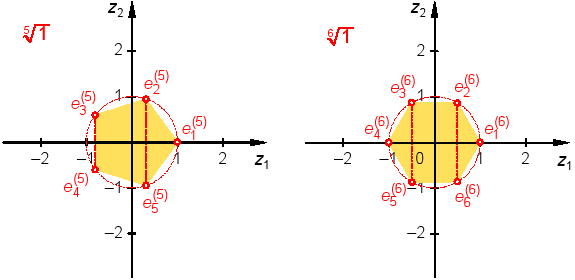
\includegraphics[width=7cm]{./bilder/einheitswurzel.png}
\end{center} \\
\end{tabular}


\textbf{12.Einheitsqurzel:} \\
$e^{(12)}_1 = 1,\;
  e^{(12)}_2 = \frac{\sqrt3}{2} + \frac12j,\;
  e^{(12)}_3 = \frac12 + \frac{\sqrt3}{2}j,\;
  e^{(12)}_4 = j,\;
  e^{(12)}_5 = -\frac12 + \frac{\sqrt3}{2}j,\;
  e^{(12)}_6 = -\frac{\sqrt3}{2} + \frac12 j,\\
  e^{(12)}_7 = -1,\;
  e^{(12)}_8 = -\frac{\sqrt3}{2} - \frac12 j,\;
  e^{(12)}_9 = -\frac12 - \frac{\sqrt3}{2}j,\;
  e^{(12)}_{10} = -j,\;
  e^{(12)}_{11} = \frac12 - \frac{\sqrt3}{2}j,\;
  e^{(12)}_{12} = \frac{\sqrt3}{2} - \frac12j$





\subsection{Nullstellen von Polynomen}
Ein complexes Polynom p(z) von Grad $n$ hat in $ \mathbb{C} $ genau $n$ Nullstellen.\\
Alle diese Nullstellen liegen in einer Kreisscheibe um den Ursprung mit dem Radius $ \sum\limits_{k=0}^{n} \left| \frac{a_k}{a_n} \right|$ \\ \\
Bei Polynomen mit reellen Koeffizienten treten nicht-reelle Nullstellen immer
als conj.-compl. Paare ($z_0$ und $\bar{z_0}$) auf. 

\skriptsubsection{Euler}{30f}
\begin{tabular}{llllll}
$\sin{\alpha} = \frac{e^{j\alpha} - e^{-j\alpha}}{2j}$ &

$\cos{\alpha} = \frac{e^{j\alpha} + e^{-j\alpha}}{2}$ &

$\tan{\alpha} = \frac{\sin \alpha}{\cos \alpha}$ & 

$ \qquad \qquad $ &

$\sinh{\alpha} = \frac{e^\alpha - e^{-\alpha}}{2} $ &

$\cosh{\alpha} = \frac{e^\alpha + e^{-\alpha}}{2} $
\end{tabular}

\skriptsubsection{Überlagerung von harmonischen Schwingungen}{32f}
$$A \cdot \sin(\omega t + \varphi) = Im[A \cdot e^{j(\omega t + \varphi)}] =
Im[\underbrace{A \cdot e^{j\varphi}}_{\text{\tiny{Complexe Amplitude}}}
\cdot \underbrace{e^{j\omega t}}_{\text{\tiny{Zeitfunktion}}}]$$
%
%Alle komplexen Schwingungen in kartesische Form umwandeln und addieren, danach
%wieder zurück in Polarform $ A_{total} \cdot e^{j\varphi}$ zurückwandeln.
%
$$ A_1 \cdot \sin(\omega t + \varphi_1) + A_2 \cdot \cos(\omega t + \varphi_2) 
 \quad \Rightarrow \quad 
 Im[A_1 \cdot e^{j(\omega t + \varphi_1)} + A_2 \cdot e^{j (\omega t + \varphi_2
 + \frac{\pi}{2})}] \quad \Rightarrow \quad 
 Im[e^{j \omega t} \cdot  (A_1 \cdot e^{j \varphi_1} + A_2 \cdot e^{j (\varphi_2
 + \frac{\pi}{2})}]$$ 
Complexe Amplituden in cartesische Form umwandeln, zusammenzählen und wieder
zurück in Polarform wandeln.
$$ Im[e^{j \omega t} \cdot  (A_{total} \cdot e^{j \varphi_{total}})] 
 \quad \Rightarrow \quad 
 Im[A_{total} \cdot e^{j (\omega t + \varphi_{total})}] 
 \quad \Rightarrow \quad 
 A_{total} \cdot \sin(\omega t + \varphi_{total})$$

%Bsp: 
%$y = y_1 + y_2 = A_1 \sin(\omega t + \varphi_1) + A_2 \underbrace{\cos(\omega t
%+ \varphi_2)}_{\text{\tiny{zu sin verwandeln}}}
%= A_1 \sin(\omega t + \varphi_1) - A_2 \sin(\omega t + (\varphi_2
%-\frac{\pi}{2}))$\\
%$= \text{Im}(\underbrace{A_1 e^{j\varphi_1}}_{\text{\tiny{$A_{1im} = A_1 \cjs
%A_1 \cdot \sin(\omega t + \varphi_1) + \varphi_1$}}} e^{j\omega t} - 
%\underbrace{A_2 e^{j(\varphi_2 - \frac{\pi}{2})}}_{\text{\tiny{$A_{2im} = A_2 \cjs
%(\varphi_2 - \frac{\pi}{2})$}}} e^{j \omega t}) 
%= (A_{1im} + A_{2im}) \sin(\omega t)$
\skriptsection{Complexe Funktionen (Abbildungen)}{37ff}
	Eine complexe Funktion hat einen 2-dimensionalen Input ($z_1$, $z_2$) und einen
	2-dimensionalen Output ($w_1$, $w_2$). \\
	Diese Abbildungen sind bis jeweils auf wenige Punkte (bei der Sinus-Funktion
	$\pm$1, etc) winkeltreu.\\
	$ f: \mathbb{D} \subseteq \mathbb{C} \mapsto \mathbb{C} \qquad z  \mapsto w = f(z)$\\
	$w_1 = \text{Re}(f(r+jc)); w_2 = \text{Im}(f(r+jc))$ 
 

	\skriptsubsection{Lineare Funktion}{41ff}
	  	\begin{minipage}{9cm}
		    $$ f : z \mapsto w = az + b \qquad (a, b \in \mathbb{C} \text{ und } a \neq0)\\$$
			- für $a = 1$ eine Translation um den Ortsvektor b \\
	    	- für $a \neq 1$ eine Drehstreckung mit dem Zentrum $\frac{b}{1-a}$, dem Drehwinkel $\arg(a)$ und dem Streckfaktor $|a|$.  
	    \end{minipage}
  		\hspace*{2cm}
  		\begin{minipage}{8cm}
      		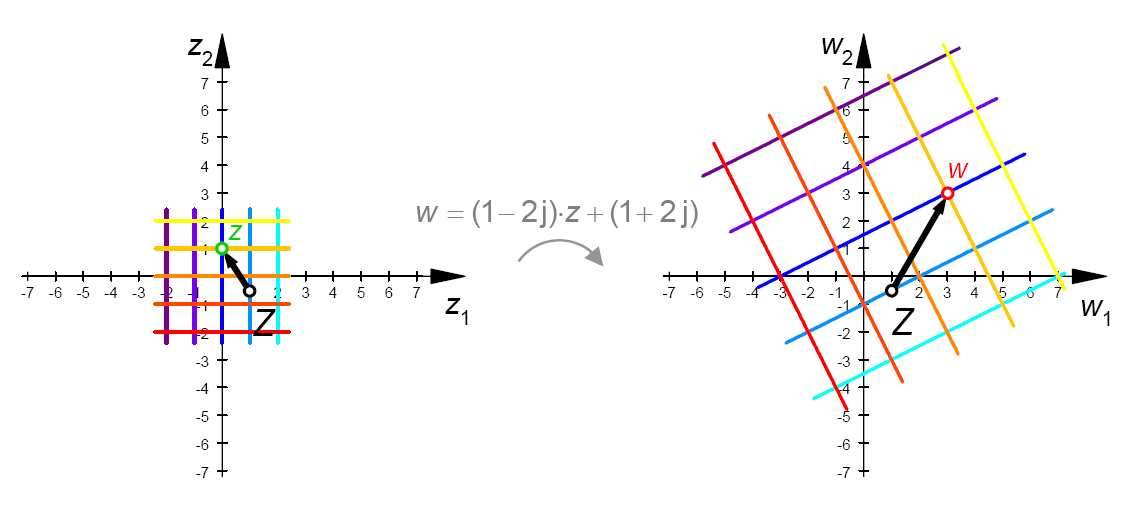
\includegraphics[width=8cm]{./bilder/LineareFunktion.png}
    	\end{minipage}

	\skriptsubsection{Quadratfunktion und Quadratwurzelfunktion}{45ff}
  		\begin{minipage}{9cm}
      		$$ f : z \mapsto w = z^2 \qquad \qquad f : z \mapsto w = \sqrt{z} $$\\
    		Bei der Quadratfunktion wird schon die rechte Hälfte der z-Ebene auf die ganze w-Ebene abgebildet (die Argumente werden verdoppelt). Daraus ergibt sich zwei bzw. mehrere Ebenen.
    	\end{minipage}
  		\hspace*{2cm}
  		\begin{minipage}{8cm}
      		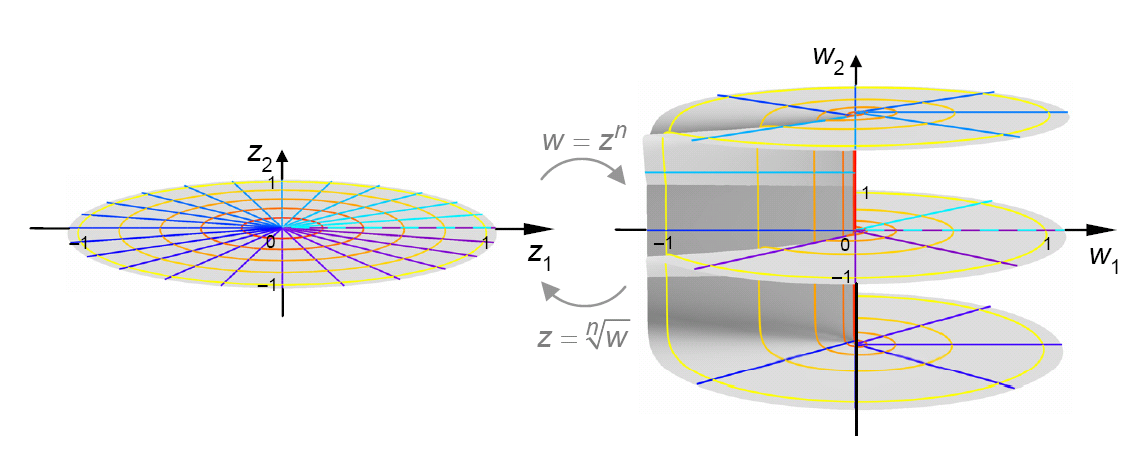
\includegraphics[width=8cm]{./bilder/RiemannischeFlaeche.png} 
      		Eine Riemanische Fläche 3.Grades
    	\end{minipage}

	\skriptsubsection{Winkeltreue}{}
		\skriptsubsubsection{differenzierbare Funktionen}{}
			Eine komplexe differenzierbare Funktion $f$ ist in allen Punkten mit $f'(z)\neq0$ eine winkeltreue Abbildung. Sie bewirkt dort lokal eine Drehstreckung mit Drehwinkel $arg\left[f'(z)\right]$ und Streckfaktor $\left|f'(z)\right|$

		\skriptsubsubsection{quadratische Funktionen}{}
			Die Quadratfunktion $f:Z\mapsto z^2$ bildet die $z$-Ebene bijektiv auf eine zweiblättirge Riemamsche Fläche ab. Sie hat die Ableitungsfunktion $f':z\mapsto 2z$ und ist deshalb überall ausser im Koordinatenursprung winkeltreu.\\
			Die Quardatwurzelfunktion $f^{-1}:w \mapsto \sqrt{w}$ ist somit ebenfals überall ausser im Koordinaten ursprung winkelreu.

	\skriptsubsection{Kehrwertfunktion und Kreisspiegelung}{51ff}
  		$$ f : z \mapsto w = \frac{1}{z}; \quad (\arg(w) = -\arg(z), |w| = \frac{1}{|z|})
  		\qquad \qquad 
  		\overline{f}: z \mapsto w = \frac{1}{\overline{z}};  \quad  
  		(\arg(w) = \arg(z), |w| = \frac{1}{|z|}) $$\\
 		Kreisspiegelung: Alle Punkte auf der z-Ebene werden am Einheitskreis gespiegelt. Geraden auf Kreise abgebildet und umgekehrt. Der Ursprungspunkt (0;0) wird auf $ \infty $ abgebildet (auf allen Winkeln zwischen $0^o-360^o$). Die Abbildungen sind im verallgemeinerten Sinn (Geraden sind Kreise mit unendlichem Radius) kreistreu. Ausserdem sind sie bis auf den Koordinatenursprung winkeltreu\\
  		\begin{minipage}{9cm}
    		\begin{tabbing}
	    		xxxxxxxxxxxxxxxxxxxxxxx\=xxxxxxxxxxxxxxxxxxxxxxxx\kill
          		- Gerade durch 0 $\Longrightarrow$ \>Fixgerade (gleiche Gerade, aber die \\ \>Punkte darauf sind anders verteilt)\\ \\
      			- Gerade nicht durch 0 $\Longrightarrow$ Kreis durch 0\\ \\ \\ \\ \\ \\ \\ \\
      			- Kreis nicht durch 0 $\Longrightarrow$ \>Spiegelung des Kreises\\ \> an dem Einheitskreis\\ \\
      			- Kreis durch 0 $\Longrightarrow$\>Gerade nicht durch 0
        	\end{tabbing}
  		\end{minipage}
  		\hspace*{2cm}
  		\begin{minipage}{6cm}
    		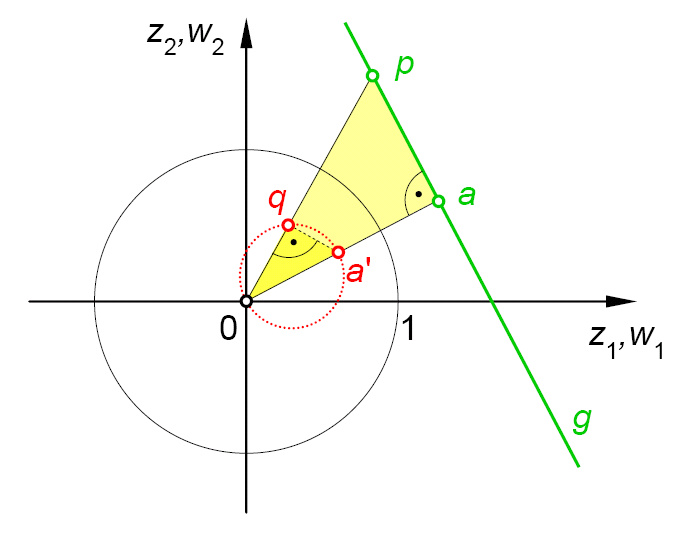
\includegraphics[width=6cm]{./bilder/GeradeKreisspiegelung.png} 
      		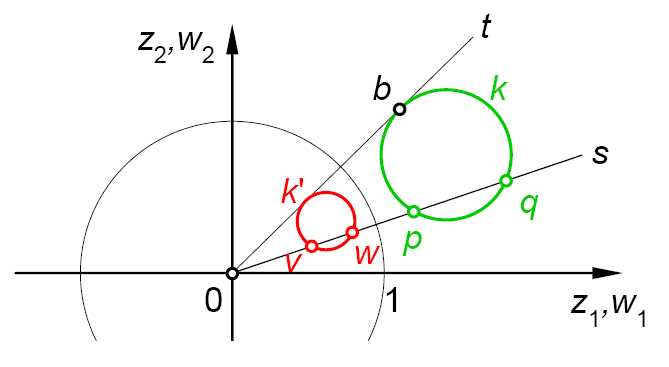
\includegraphics[width=6cm]{./bilder/KreisKreisspiegelung.png}
    	\end{minipage}

	\skriptsubsection{Möbiustransformation}{57ff}
  		\begin{minipage}{10cm}
    		$$ f : z \mapsto w = f(z) = \frac{az + b}{cz + d}$$
    		$$(a, b, c, d \in 
    		\mathbb{C} \text{ mit } c \neq 0 \text{ und } ad - bc \neq 0) $$
    		Die Möbiustransformation ist eine Verkettung einer linearen Funktion, der Kehrwertfunktion und einer weiteren linearen Funktion. \\
    		Diese Transformationen sind winkel- und kreistreu. Die Umkehrfunktion ergibt wieder eine Möbiustransformation. \\
    		Eigentlich besitzt diese Funktion nur drei Parameter da man den Bruch $\frac{az + b}{cz + d}$ stets so kürzen kann dass einer der vier Parameter 1 ist. Durch die 3 Freiheitsgrade kann man unterschiedlichste Kriterien vorgeben und damit komplizierte Umformungen machen, wie im Bild gezeigt wird:  
  		\end{minipage}
  		\hspace*{2cm}
  		\begin{minipage}{7cm}
    		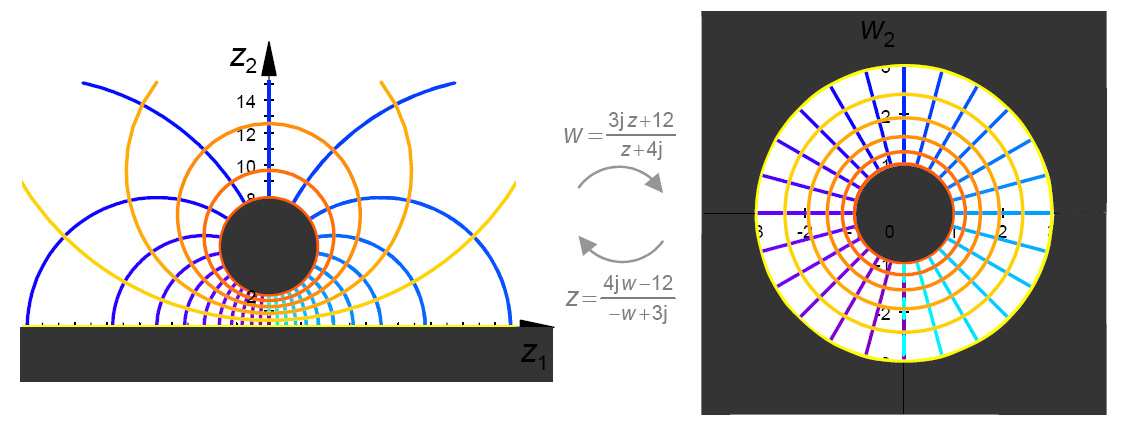
\includegraphics[width=7cm]{./bilder/Moebiustransformation.png} 
  		\end{minipage}

	\skriptsubsection{Joukowski-Funktion}{60ff}
  		\begin{minipage}{10cm}
    		$$ f : z \mapsto w = z + \frac{1}{z}  $$
    		Die Funktion ist winkeltreu bis auf $\pm$2\\
    		Wenn man einen Kreis, der nicht ganz im Zentrum steht transformiert ergibt sich ein Flügelprofil
  		\end{minipage}
  		\hspace*{2cm}
  		\begin{minipage}{7cm}
    		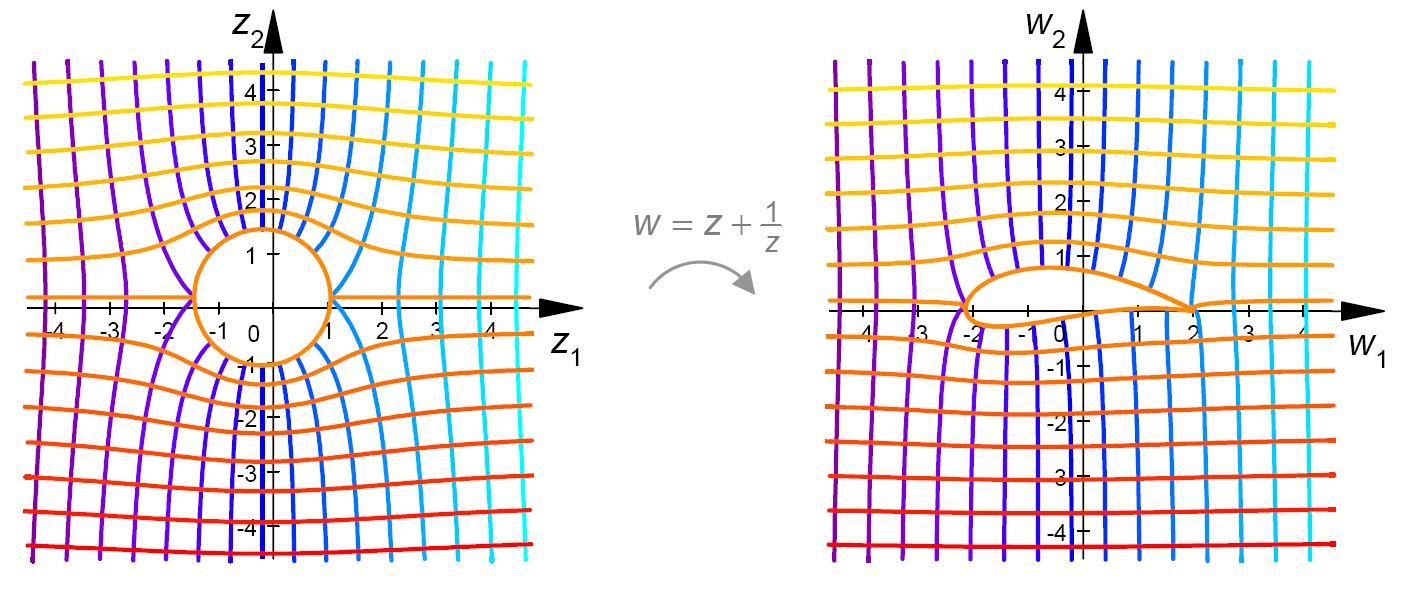
\includegraphics[width=7cm]{./bilder/joukowskiFunktion.png} 
  		\end{minipage}
  		
	\skriptsubsection{Exponentialfunktion}{64ff} 
  		\begin{minipage}{9cm}
    		$$ f : z \mapsto w = e^z $$
    		Waagrechte Gitternetzlinen gehen gemäss der obigen Gleichung in Strahlen über, die im Koordinatenursprung beginnen, senktrechte Gitternetzlinien in Kreise um den Koordinatenursprung. Die e$^z$-Funktion ist periodisch, deshalb braucht es eine Riemansche Fläche\\ \\
		    Mit dieser Funktion kann man das Feld bei den Rändern des Plattenkondensator berechnen 
  		\end{minipage}
  		\hspace*{2cm}
  		\begin{minipage}{7cm}
    		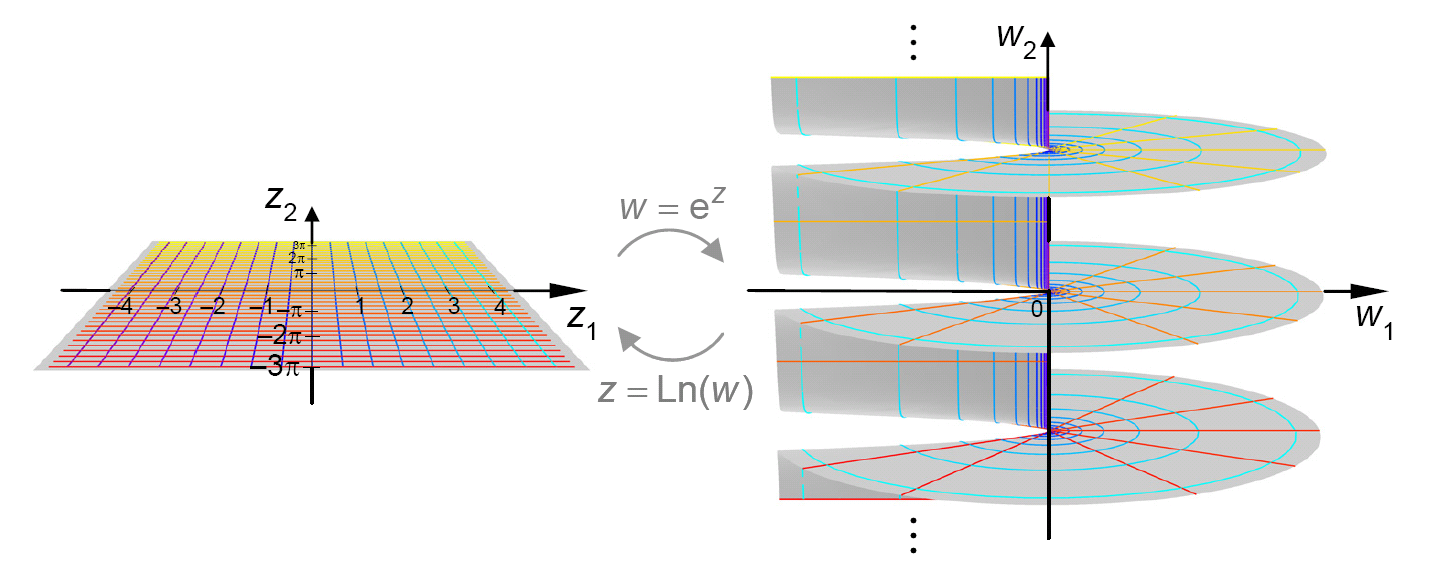
\includegraphics[width=7cm]{./bilder/ehochz.png} 
    		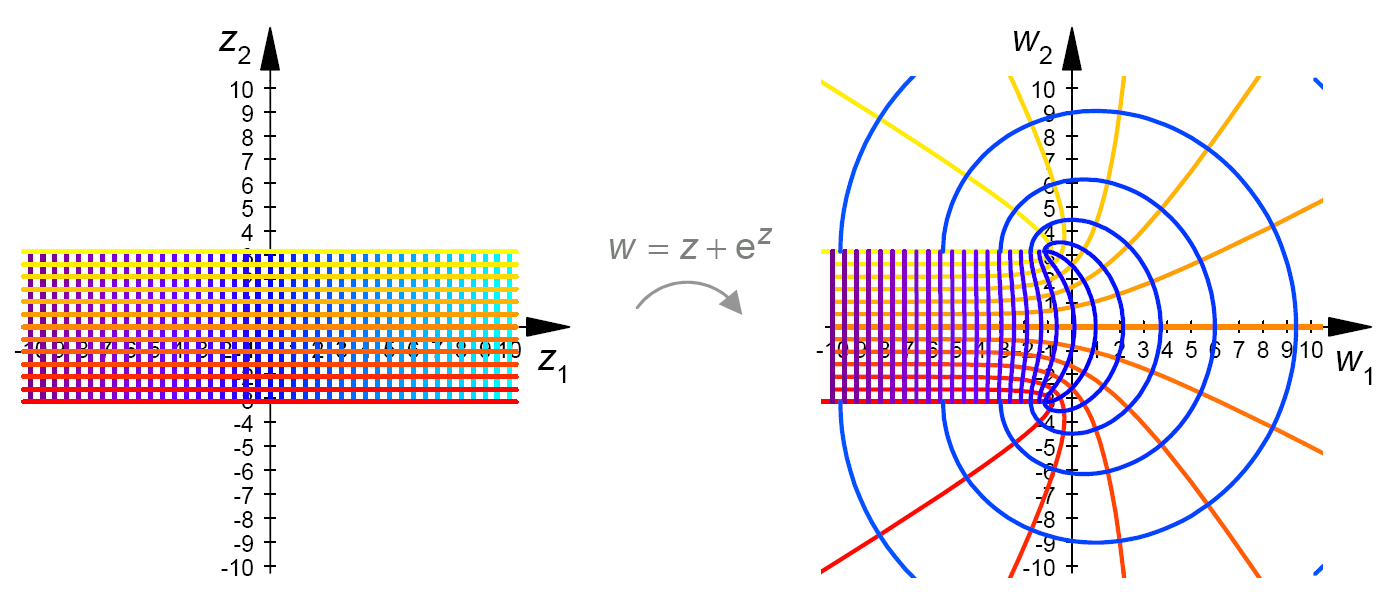
\includegraphics[width=8cm]{./bilder/plattenkondensator.png}    
  		\end{minipage}

	\skriptsubsection{Sinus-Funktion}{67f}
   		\begin{minipage}{10cm}
    		$$ f : z \mapsto w = \sin(z) $$    
    		Die Sinusfunktion ist ausser bei den Punkten $z = \frac{\pi}{2}+ k\pi (k \in \mathbb{Z}))$ winkeltreu
  		\end{minipage}
  		\hspace*{2cm}
  		\begin{minipage}{7cm}
    		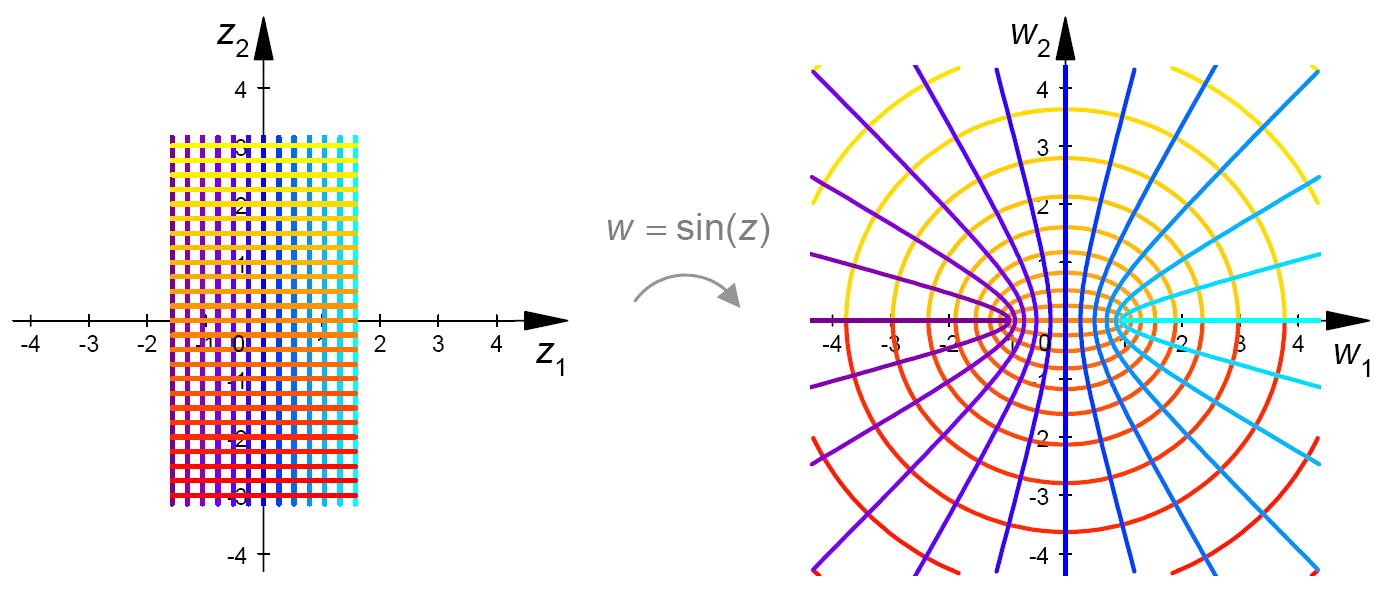
\includegraphics[width=7cm]{./bilder/sinus.png}   
  		\end{minipage}
 
		\subsection{Kreisgleichung}
			Die Lösungen von z bilden einen Kreis in der mit dem Radius $r$ um den Mittelpunkt $M=(m_x, m_y) \Rightarrow m=m_x + j m_y$. \\
			$$|z-m| = r; \qquad 
			(z-m)(\overline{z} - \overline{m}) = r^2; \qquad 
			z\overline{z} - \overline{m}z - m\overline{z} + m\overline{m} = r^2$$
			$$ \text{Parameterform: } f(t) = m + r \cdot e^{jt}, \quad \text{mit } (0 \leq t \leq 2 \pi) $$
\skriptsection{Fourierreihen}{67ff}
    \skriptsubsection{Orthogonalitätsbeziehungen der Basisfunktionen}{75}
        \begin{tabular}{lll}
            $\int\limits_0^T \cos(n\omega t)\cdot \cos(m\omega t)dt=
            \begin{cases}
            T,\ n=m=0\\
            \frac{T}{2},\ n=m>0\\ 
            0,\ n\neq m\\
            \end{cases}$ &
            $\int\limits_0^T \sin(n\omega t)\cdot \sin(m\omega t)dt=
            \begin{cases}
            \frac{T}{2},\ n=m\\
            0,\ n\neq m\\
            \end{cases}$&
            $\int\limits_0^T \cos(n\omega t)\cdot \sin(m\omega t)dt=0$
        \end{tabular}
  \skriptsubsection{Allgemeine Form}{79}
    Eine periodische Funktion f mit Periode $T>0$, lässt sich durch eine Reihe von
    Sinus- und Kosinusfunktionen darstellen, deren Frequenzen ganzzahlige 
    Vielfache der Grundfrequenz $\omega = 2\pi / T$ sind:
    $$ f(t)=\frac{a_0}{2} + \sum_{n=1}^\infty (a_n \cdot \cos(n \omega t) + b_n
    \cdot \sin(n\omega t))$$
    Die Koeffizienten der Entwicklung von $f(t)$ sind:
    $$ a_n=\frac{2}{T}\int\limits_{0}^{T} f(t) \cdot \cos(n\omega t)\,
    \mathrm{d}t \quad (n=0,1,2,3,\ldots) \qquad \qquad
    b_n=\frac{2}{T}\int\limits_{0}^{T} f(t) \cdot \sin(n\omega t)\, \mathrm{d}t \quad (n=1,2,3,\ldots) $$
    Der erste Summand der Reihe $a_0/2$ ist der Gleichstromanteil (Mittelwert) von
    $f(t)$ im Intervall $(0,T)$

  \skriptsubsection{Komplexwertige Darstellung der Fourierreihen}{95ff}
    $$f(t) = \sum\limits_{k = -\infty}^{\infty} c_k \cdot e^{j k \omega t} \qquad \text{mit} \qquad c_n=\overline{c_{-n}}=\frac{1}{T}\int_0^T{f(t)\cdot e^{-jn\omega t}dt}$$
    \subsubsection{Umrechnungsformeln}
      $$c_n=\overline{c_{-n}}=\frac{a_n-jb_n}{2} (n=0,1,2,3,\ldots\text{ wobei }b_0=0)\qquad
      \left.
      \begin{array}{l} 
        a_n=2 \cdot \text{Re}(c_n)\\
        b_n=-2 \cdot \text{Im}(c_n)
      \end{array}
        \right\} 
        \quad
      (n=0,1,2,3,\ldots, b_0 = 0)$$

  \skriptsubsection{LTI-Systeme}{72} 
      \subsubsection{Linear}
      \begin{tabular}{llll}
            \textbf{Aus}: &
            $f(t)\to \fbox{S}\to F(t)$ &
            und &
            $g(t)\to \fbox{S}\to G(t)$ \\
            \textbf{folgt} &
            $f(t)+g(t)\to \fbox{S}\to F(t)+G(t)$ &
            und &
            $r\cdot f(t)\to\fbox{S}\to r\cdot F(t)$ \\
        \end{tabular}
        \subsubsection{Zeitinvarianz}
        \begin{tabular}{llll}
            \textbf{Aus} &
            $f(t)\to \fbox{S}\to F(t)$ &
            \textbf{folgt} &
            $f(t+t_0)\to \fbox{S}\to F(t+t_0)$\\
        \end{tabular}
  \skriptsubsection{Sätze zur Berechnung der Koeffizienten}{80ff}
    \skriptsubsubsection{Symmetrie}{80f}
    \begin{tabular}{ll}
        Falls $f(t)$ \textbf{gerade} ($ f(-t)=f(t) $) ist 
        & $\quad \Longrightarrow \quad 
      b_n = 0, \quad a_n = \frac{4}{T} \int\limits_0^{\frac{T}{2}} f(t) \cdot
      \cos(n \omega t) \mathrm{d}t$ \\
      Falls $f(t)$ \textbf{ungerade} ($ f(-t)=-f(t) $) ist
      &$\quad \Longrightarrow \quad a_n = 0, \quad b_n =  \frac{4}{T} 
      \int\limits_0^{\frac{T}{2}} f(t) \cdot \sin(n \omega t) \mathrm{d}t$
        \end{tabular}
       
    \skriptsubsubsection{Linearität}{82}
      $h(t) = r \cdot f(t) + s \cdot g(t) \quad \Longrightarrow \quad a_n^{(h)} = r \cdot
      a_n^{(f)} + s \cdot a_n^{(g)}, \quad b_n^{(h)} = r \cdot b_n^{(f)} + s \cdot b_n^{(g)}$
      
    \skriptsubsubsection{Zeitstreckung/-stauchung ("Ahnlichkeit)}{83}
      $g(t) = f(r \cdot t) $ (mit $ 0 < r \in \mathbb{R}$ ) $\quad \Longrightarrow\quad  
      a_n^{(g)} = a_n^{(f)}, \quad b_n^{(g)} = b_n^{(f)} $ \quad $T^{(g)} = \frac{T^{(f)}}{r}$.
      
    \skriptsubsubsection{Zeitverschiebung}{84} 
    \label{Fourier_Zeitverschiebung}
    $g(t)=f(t+t_0)$
    $\qquad
    \begin{array}{l}
           a_n^{(g)}=\cos(n\omega t_0)\cdot a_n^{(f)}+\sin(n\omega t_0)\cdot b_n^{(f)}\\
           b_n^{(g)}=-\sin(n\omega t_0)\cdot a_n^{(f)}+\cos(n\omega t_0)\cdot b_n^{(f)}\\
           c_n^{(g)}=e^{jk \omega t_o} \cdot c_k^{(f)}
        \end{array}$
        $\quad
    \begin{array}{l}
           (n=0,1,2,\ldots)\\
           (n=1,2,3,\ldots)\\
           (k \in \mathbb{Z})
        \end{array}$ \\
    
\skriptsubsection{Integral und Differential}{88}
Falls die T-periodische Funktion $f$ (auf ganz $\mathbb{R}$) zweimal stetig differenzierbar ist und die Fourierkoeffizienten $a_n$ und $b_n$ besitzt, so gilt:
$$ f'(t) = \sum\limits_{n=1}^{\infty} [b_n n \omega \cdot \cos{(n \omega t)} - a_n n \omega \cdot \sin{(n \omega t)}]
\qquad \qquad \int\limits_0^t f(\tau) d\tau = \sum\limits_{n=1}^{\infty} \frac{b_n}{n \omega} + 
\frac{a_0}{2} t + \sum\limits_{n=1}^{\infty}
[\frac{a_n}{n \omega} \cdot \sin{(n \omega t)} - \frac{b_n}{n \omega} \cdot \cos{(n \omega t)}] $$

\skriptsubsection{Gibbs'sches Phänomen}{92f}
Die Fourier-Reihen schwingen bei Unstetigkeitsstellen über. Die Höhe des
Überschwingers lässt sich so berechnen:

\begin{figure}[htbp]
  \begin{minipage}[b]{8cm}
$$\frac{1}{\pi}\int\limits_0^\pi \frac{\sin t}{t}\, \mathrm dt - \frac{1}{2} =
0{,}089490\dots$$ \\
  \end{minipage}
  \begin{minipage}[b]{8cm}
    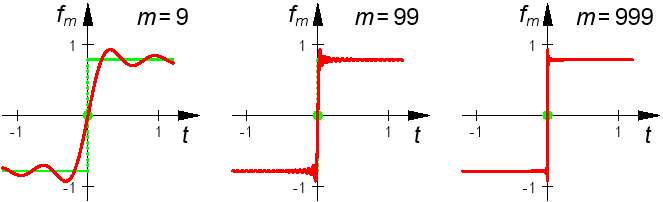
\includegraphics[width=8cm]{./bilder/gibssches_phaenomen.png}  
  \end{minipage}
\end{figure}

Bei Unstetigkeitsstellen konvergiert die Fourierreihe gegen:\\
$\frac{f(t_0-0)+f(t_0+0)}{2}$

\skriptsubsection{Frequenz-, Amplituden- und Phasengang}{72}
$ \text{Frequenzgang eines Systems: } H(\omega) = A(\omega) \cdot e^{j \Phi(\omega)} \qquad 
\text{ Amplitudengang: } A(\omega) = |H(\omega)| \qquad \text{ Phasengang } \Phi(\omega) = arg[H(\omega)] $ \\ \\
Die komplexe Funktion $H(\omega)$ der reellwertigen Frequenz $\omega$ enthält zugleich die Informationen über 
die Veränderung der Amplitude und der Phasenverschiebung des Systems S bei der betrachteten Frequenz $\omega$.
$$f(t) = Im[z(t)] \to \fbox{S}\to F(t) = Im[z(t) \cdot H(\omega)] \qquad \text{ oder } 
\qquad f(t) = Re[z(t)] \to \fbox{S}\to F(t) = Re[z(t) \cdot H(\omega)]$$
Je nach Eingangssignal wird der Real- oder der Imaginärteil behandelt: 
$ f(t) = 
    \left\{
    \begin{array}{l}
           sin(n t) = Im[e^{j \cdot n t}]\\
           cos(n t) = Re[e^{j \cdot n t}]
        \end{array}
    \right\}
\Longrightarrow
z(t) = e^{j \cdot n t}
$ \\

Somit kann die Antwort des Systems mittels einer komplexen Multiplikation mit der Hilfsfunktion $z(t)$ berechnet werden.

\section{Spektren}
\subsection{Spektraldarstellungen}

\begin{figure}[htbp]
  \centering
  \begin{minipage}[b]{5.5cm}
    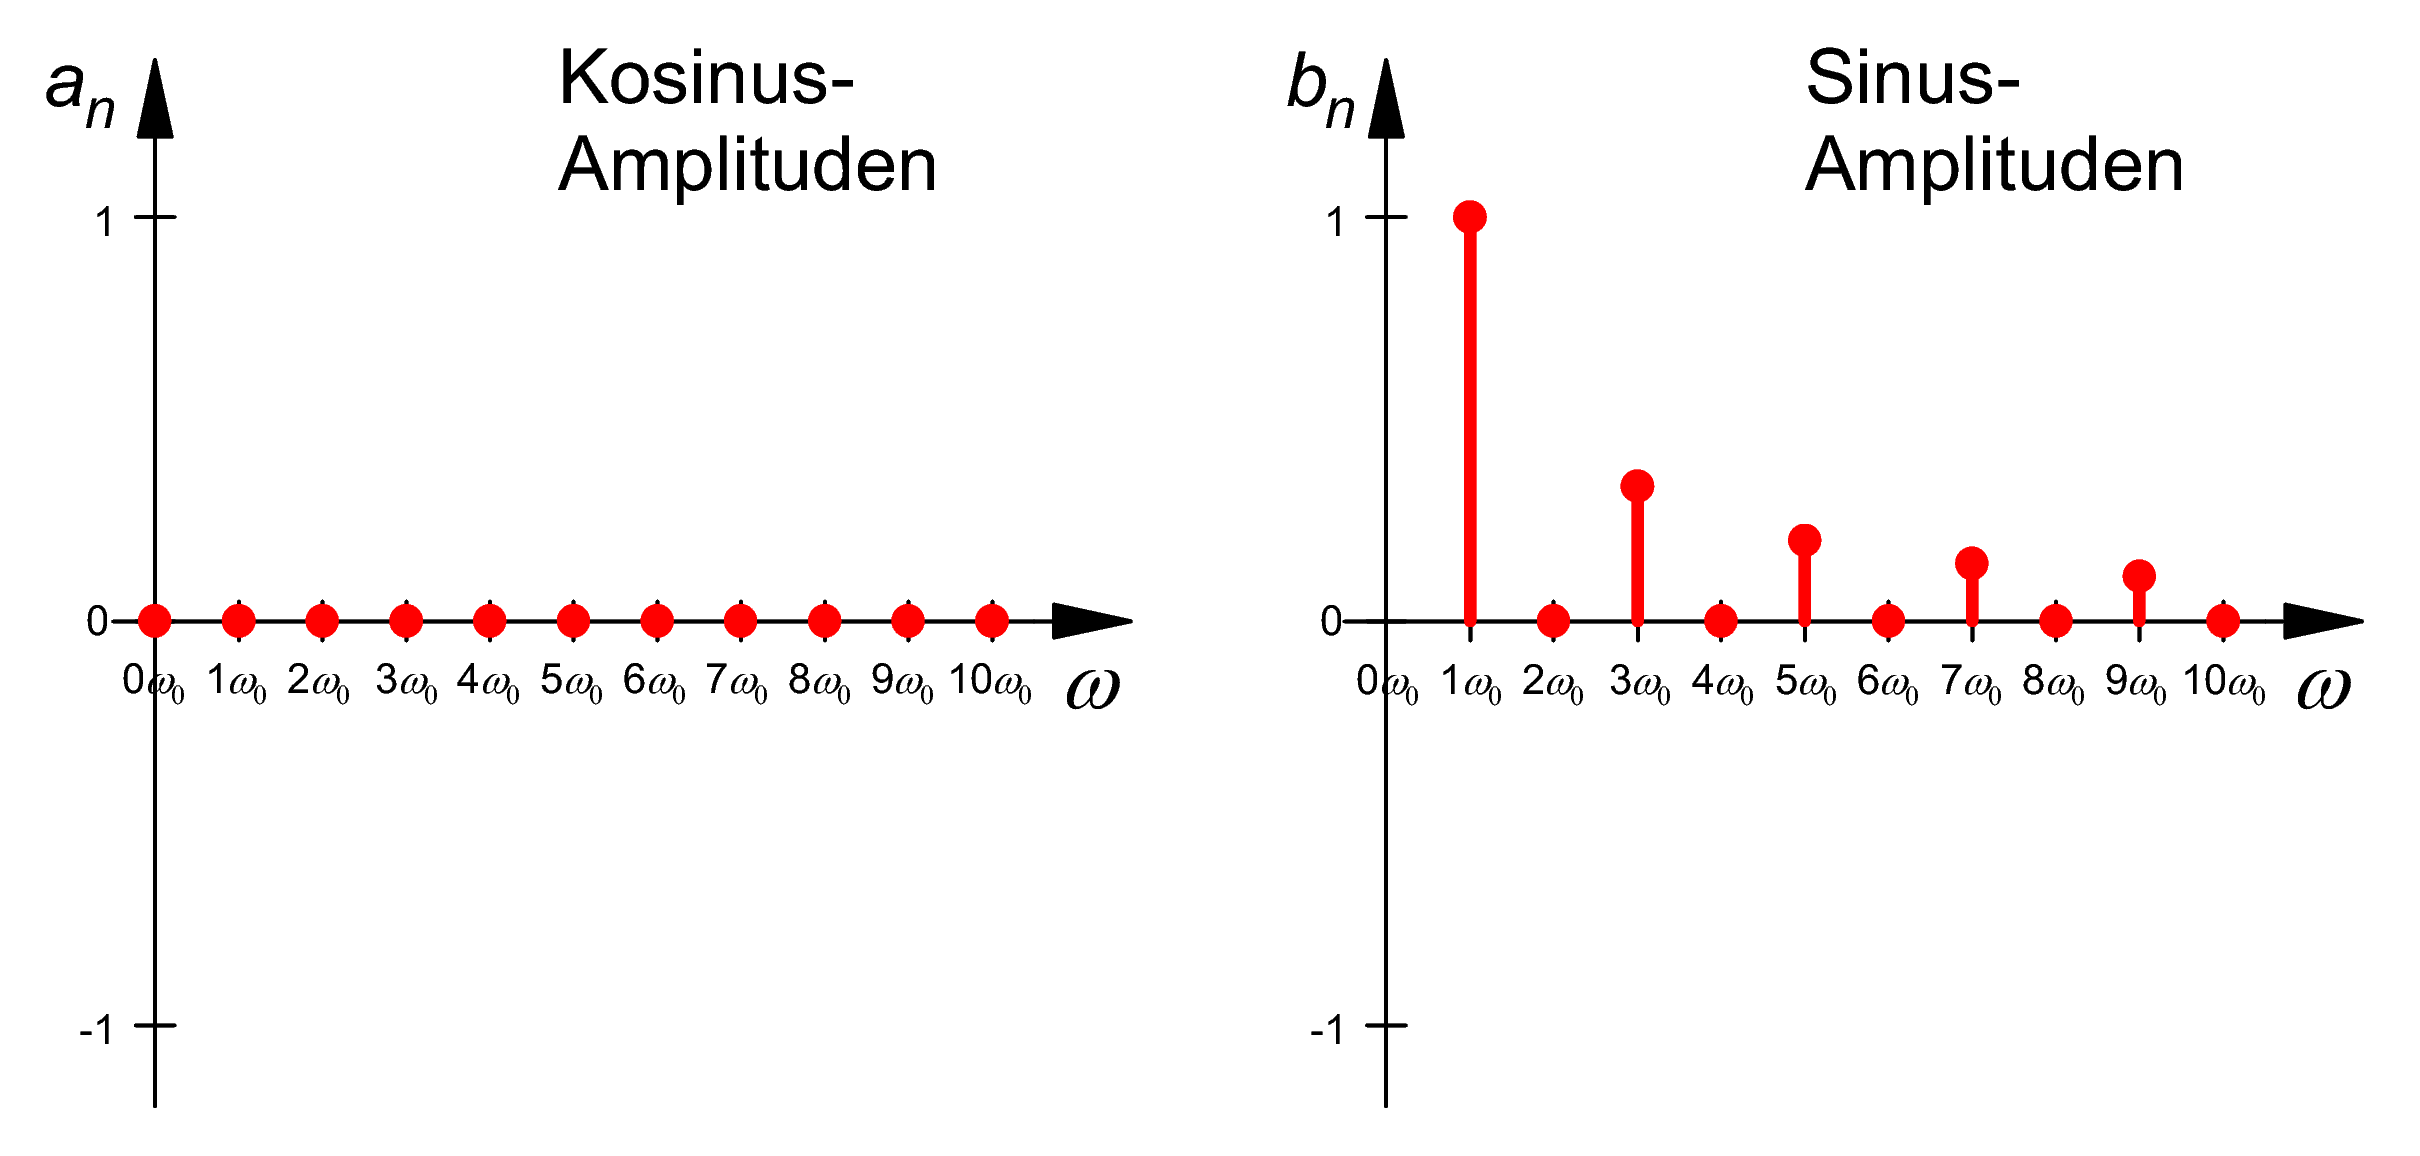
\includegraphics[width=5.5cm]{./bilder/spektren_cossin.png}
    \caption{Kosinus- und Sinusamplitudendiagramm} 
  \end{minipage}
  \hspace{1cm}
  \begin{minipage}[b]{5.5cm}
    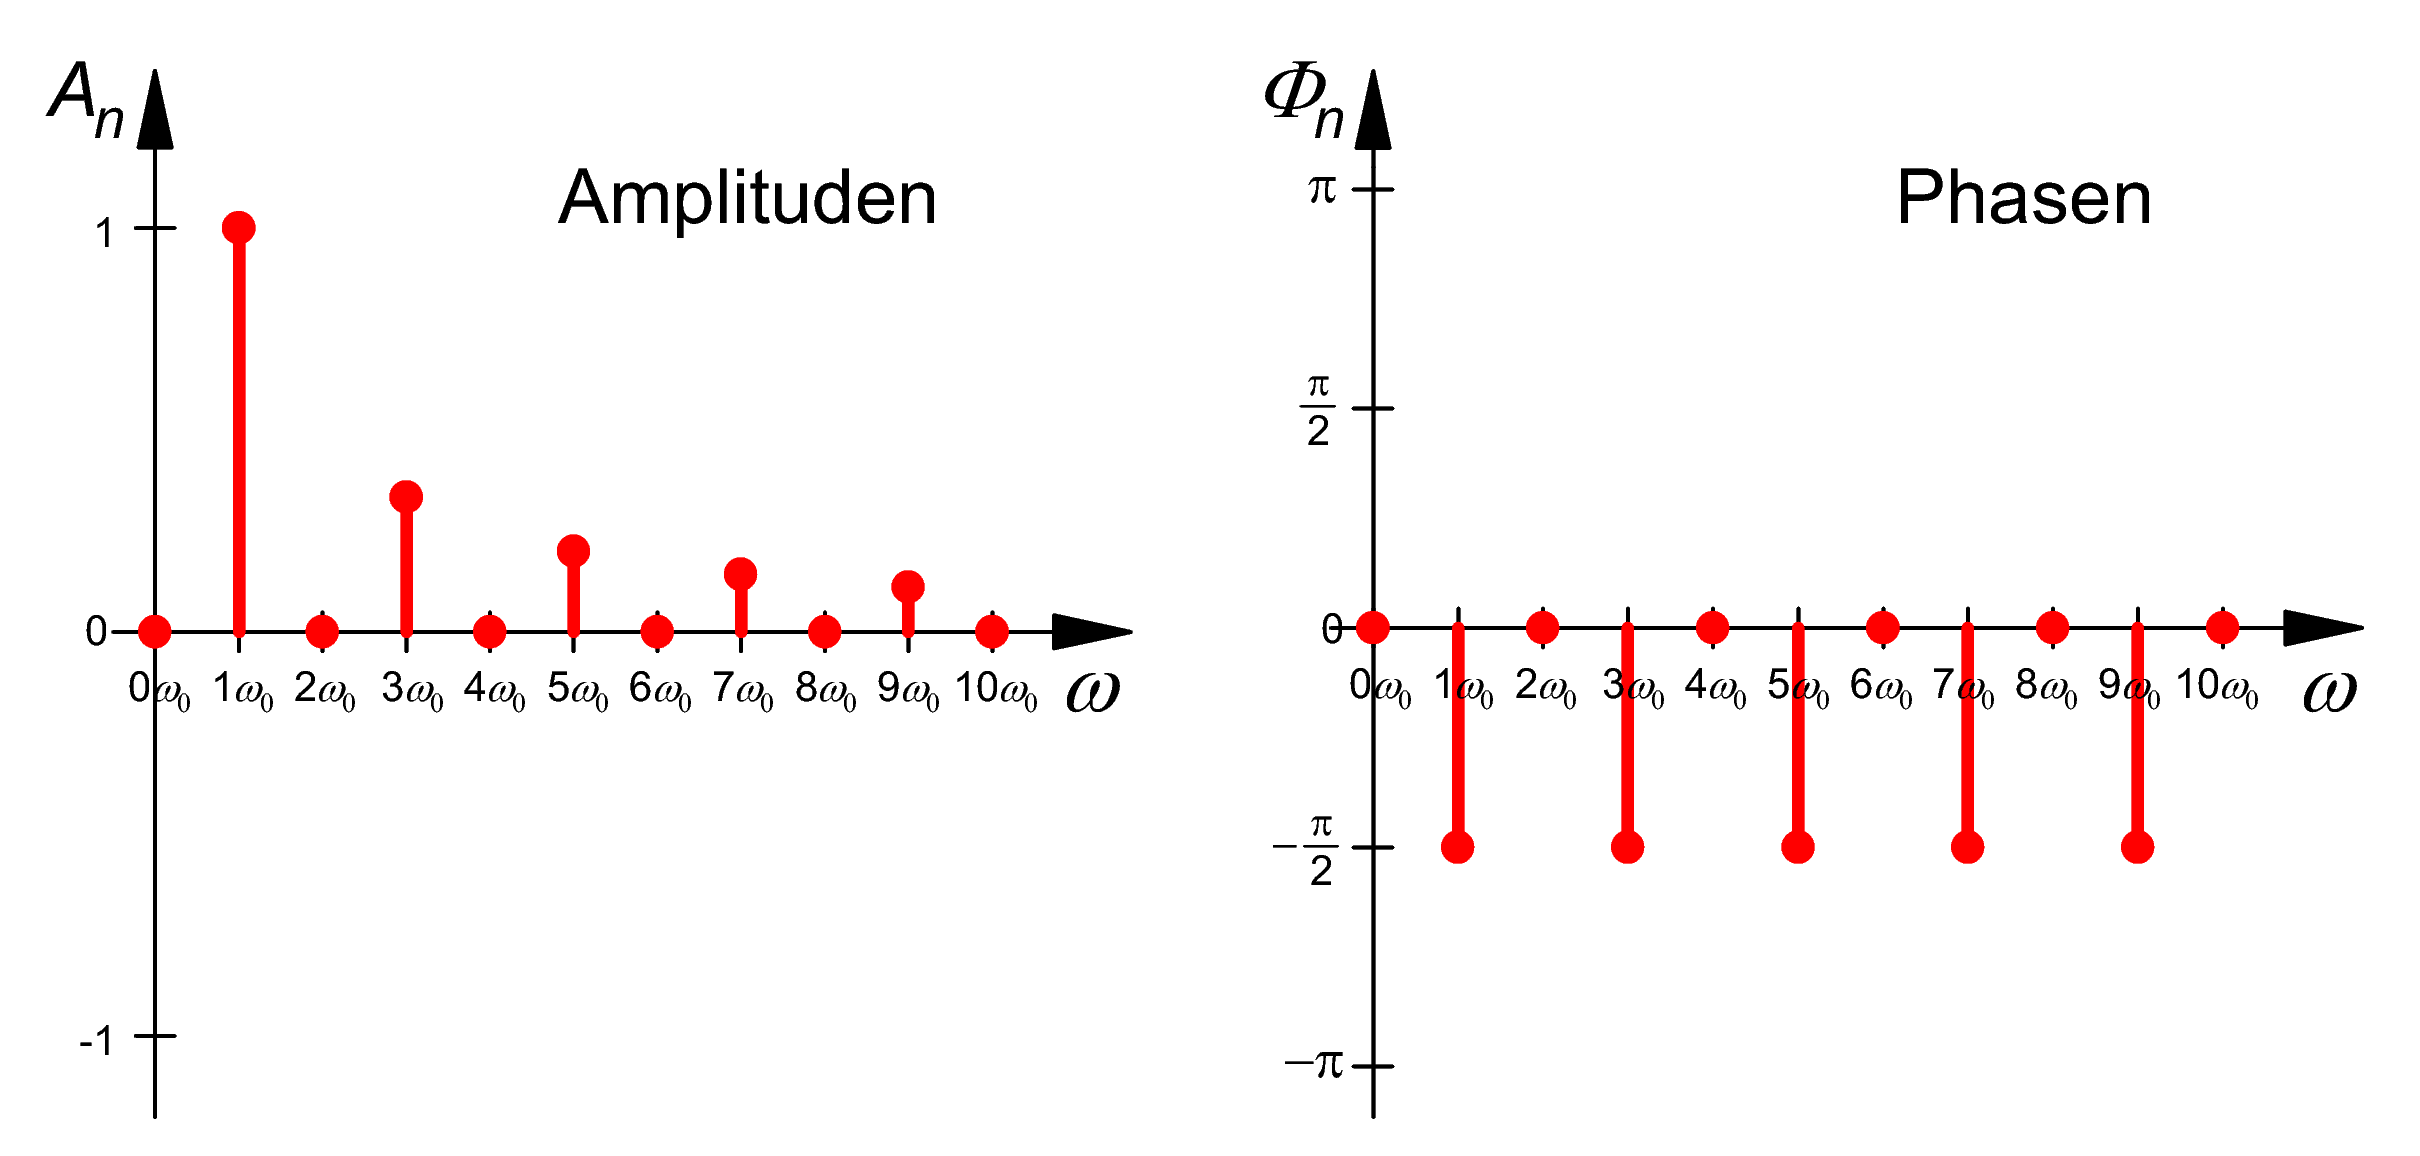
\includegraphics[width=5.5cm]{./bilder/spektren_einseitig.png} 
    \caption{Einseitiges Amplituden-/Phasendiagramm} 
  \end{minipage}
  \hspace{1cm}
  \begin{minipage}[b]{5.5cm}
    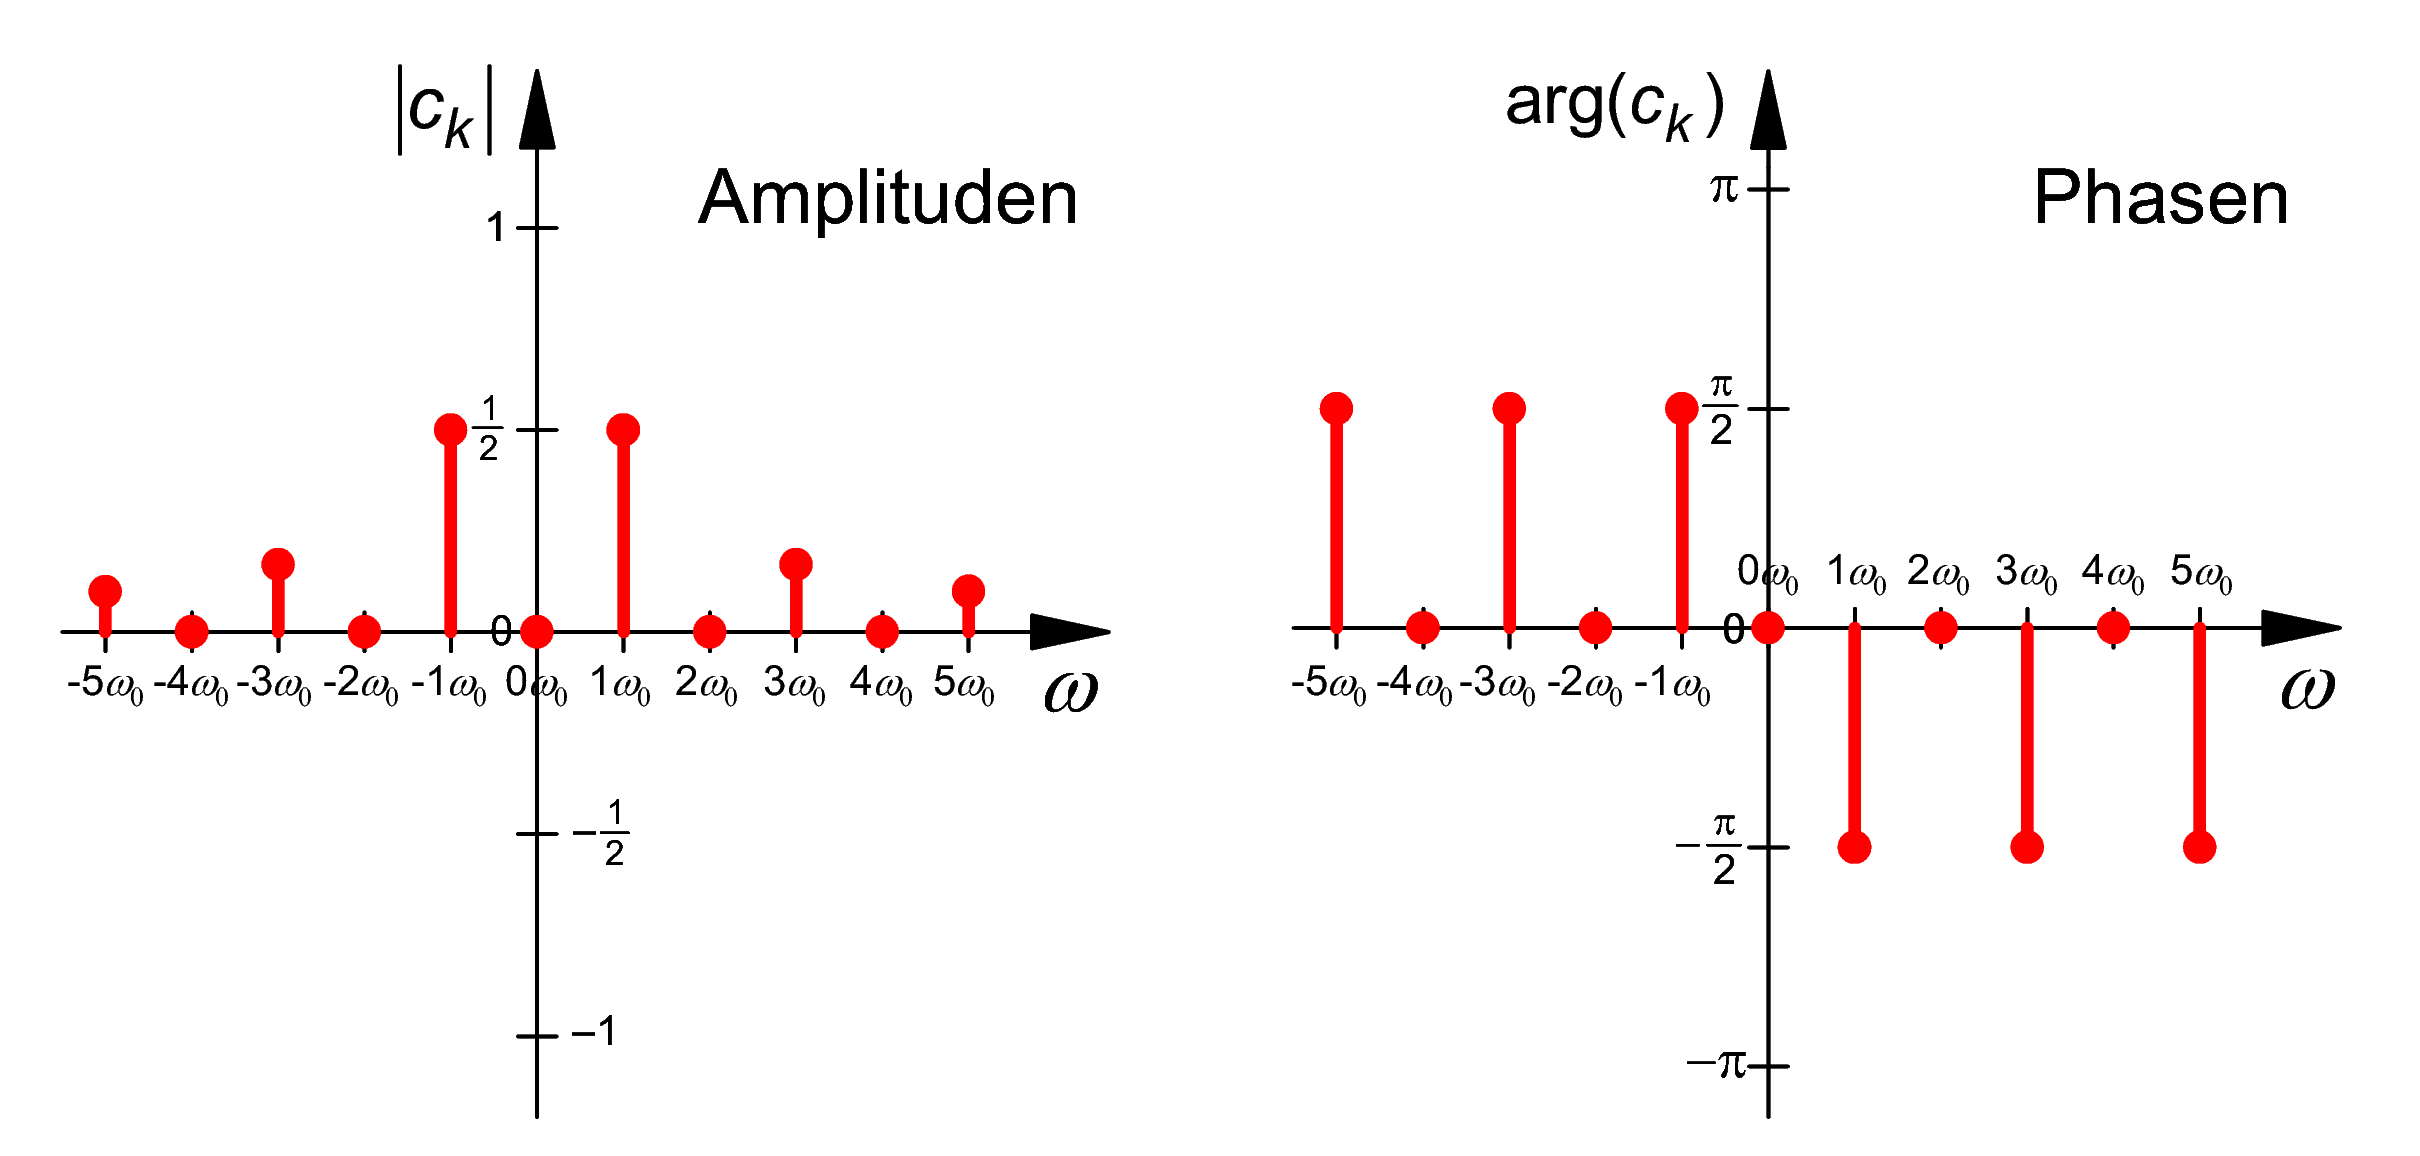
\includegraphics[width=5.5cm]{./bilder/spektren_zweiseitig.png} 
    \caption{Zweiseitiges Amplituden-/Phasendiagramm} 
  \end{minipage}
\end{figure}

\subsubsection{(1) Kosinus- und Sinusamplitudendiagramm} 
Reelle Fourierkoeffizienten ($a_n, b_n$) können direkt abgelesen werden. 
Bei einer Phasenverschiebung ändern sich jedoch die Koeffizienten grafisch nicht nachvollziehbar. \\
Diese Darstellung hat gegenüber den anderen zwei mehr Nachteile und wird daher eher selten genutzt.

\subsubsection{(2) Einseitiges Amplituden-/Phasendiagramm}
\begin{tabular}{ll}
	Amplitude $A$: &
 	$A_n = |a_n - j \cdot b_n| = \sqrt{a_n^2 + b_n^2}$ \text{ oder } $A_n =
	2 \cdot |c_n|$ \\
	
	Phase $\varphi$: &
	$\varphi_n = \arg(a_n - j \cdot b_n) \text{ oder } \varphi_n = \arg(c_n) $ \\
	
	Spezialfall: $n = 0$ &
	$A_0 = |\frac{a_0}{2}| \text{und} \varphi_0 = 
	\begin{cases}
		0 & a_0 \geq 0 \\
		\pi & a_0 < 0
	\end{cases}$ \\
	$c_n$ aus $A$ und $\varphi$: &
	$c_n = \frac{1}{2}A_n \cdot e^{j \varphi n}$\\	
\end{tabular}


\subsubsection{(3) Zweiseitiges Amplituden-/Phasendiagramm (komplexes Spektrum)} 
Amplitudendiagramm ist achsensymmetrisch wegen $ c_n=\overline{c_{-n}} $. Phasendiagramm ist punktsymmetrisch. \\
Ähnlichkeit mit Einseitigem: $|c_k| = \frac{1}{2}A_k $ und $\arg(c_k) =
\varphi_k$ für alle $ n \geq 0$.

\subsection{Spezialfälle}
\begin{tabular}{ll}
  Funktion f gerade 
  & (1) Sinusamplitudendiagramm überall 0 \\
  & (2,3) Phasendiagramm enthält nur die Werte $0$ und $\pi$ \\
  Funktion f ungerade
  & (1) Kosinusamplitudendiagramm überall 0 \\
  & (2,3) Phasendiagramm enthält nur die Werte $\pm \frac{\pi}{2}$ (oder $0$ falls Amplitudenwert $=0$) \\
  "Ahnlichkeit $g(t) = f(r \cdot t) $
  & (1,2,3) Das Spektrum von $g$ ist das horizontal mit den Faktor $r$ gestreckte Spektrum vom $f$. \\
  Zeitverschiebung $g(t) = f(t + t_0) $
  & (1) \verweis{Fourier_Zeitverschiebung}{Zeitverschiebung} \\
  & (2,3) Amplitudendiagramme sind identisch. \\
  & (2,3) Phasendiagramme: Die Sälule der Frequenz $k \omega_0$ wächst um $k\omega_0 t_0$. \\
  Weisses Rauschen
  & "Uberlagerung von Schwingungen aller möglichen Frequenzen \\
  & mit gleichen Amplituden und zufälligen Phasen. 
\end{tabular}
\skriptsection{DFT - Diskrete Fourier Transformation}{109}
\subsection{Definitionen}
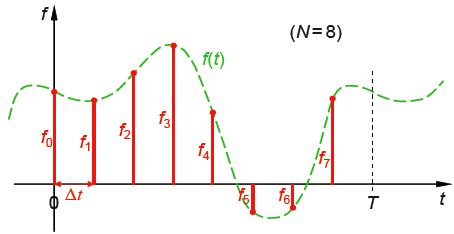
\includegraphics[width=5cm]{./bilder/abtastung.png}

\subsubsection{Diskrete komplexe Fourierkoeffizienten}
$\hat{c_k}$ sind die diskreten Fourierkoeffizienten die zu den (reellen
Abtastwerten $f_0, f_1,\ldots,f_{N-1}$) gehören\\
$$\hat{c_k}=\frac{1}{N}\sum\limits_{n=0}^{N-1}f_n\cdot e^{-\frac{2\pi j}{N}\cdot
kn}$$
Kompakte Darstellung mit der Matrix W:
$\begin{pmatrix}
 \hat{c_0}\\\hat{c_1}\\\hat{c_2}\\\hat{c_3}
\end{pmatrix}$
$=\frac{1}{N}$
$\begin{pmatrix}
 w^0w^0w^0w^0\\w^0w^1w^2w^3\\w^0w^2w^4w^6\\w^0w^3w^6w^9
\end{pmatrix}$
$\cdot$
$\begin{pmatrix}
 f_0\\f_1\\f_2\\f_3
\end{pmatrix}$
wobei $w=e^{-\frac{2\pi j}{N}}$

\subsubsection{Rechenaufwand DFT / FFT}
Der Rechenaufwand für die DFT ist proportional zu $N^2$ 
hingegen ist er bei der Fast Fourier Transform (FFT) nur $N\cdot log(N)$.

\skriptsubsection{Eigenschaften der Diskreten Fouriertransformation}{112}
\subsubsection{Alias-Effekt}
Mit $\hat{c_k}(\hat{c_0},\ldots,\hat{c_N-1})$ kennt man alle disktreten Fourierkoeffizienten. Es gilt:
$\hat{c_k}=\sum\limits_{l=-\infty}^{\infty}c_k+l\cdot N \quad l\in Z$

\subsubsection{Nyquist-Shannon-Abtasttheorem}
Ein Signal muss mit mindestens der doppelten Frequenz seines höchstfrequentigen Anteils abgetastet werden.

\skriptsubsection{Inverse Diskrete Fouriertransformation iDFT}{116}
\subsubsection{Abtastwerte berechnen}
Die N diskreten Fourierkoeffizienten lassen sich mit der iDFT wieder auf ihre Abtastwerte $f_n$ zurückführen.
$$f_n=\sum\limits_{k=0}^{N-1}(\hat{c_k}\cdot e^{\frac{2\pi j}{N}\cdot nk})$$
\subsubsection{Kontinuirliche Funktion berechnen}
Die N diskreten Fourierkoeffizienten lassen sich auch auf die kontinuirliche Funktion $f(t)$ zurückführen.
$$t\mapsto \sum\limits_{k=0}^{N-1}(\hat{c_k}e^{jk\omega_0t})$$ 
ist eine Funktion die diese diskreten Fourierkoeffizienten besitzt.
für $k=1,2,\ldots,\frac{N}{2}$ so ist auch 
$$t\mapsto\hat{c_k}+\sum\limits{k=1}{\frac{N}{2}-1}[2 
Re(\hat{c_k}e^jk\omega_0t)]+\hat{c_\frac{N}{2}}\cdot \cos(\frac{N}{2}\omega_0t)$$
eine reelle Funktion mit halb so grossen höchsten Frequenzen. 

\label{LastPage}
\section{Wichtige Formeln}

$\sin^2(b)+\cos^2(b)=1 \qquad \tan(b)=\frac{\sin(b)}{\cos(b)}$
  
  
\subsection{Funktionswerte für Winkelargumente}
  \renewcommand{\arraystretch}{1.5}
  \begin{minipage}{5cm}
    \begin{tabular}[c]{ |c|c||c|c|c| }
        \hline
      deg & rad & sin & cos & tan\\
      \hline
      0\symbol{23} & 0 & 0 & 1 & 0\\
      \hline
      30\symbol{23} & $\frac{\pi}{6}$ & $\frac{1}{2}$ & $\frac{\sqrt{3}}{2}$ &
      $\frac{\sqrt{3}}{3}$\\
      \hline
      45\symbol{23} & $\frac{\pi}{4}$ & $\frac{\sqrt{2}}{2}$ & $\frac{\sqrt{2}}{2}$
      & 1\\
      \hline
      60\symbol{23} & $\frac{\pi}{3}$ & $\frac{\sqrt{3}}{2}$ & $\frac{1}{2}$ &
      $\sqrt{3}$\\
      \hline      
    \end{tabular}     
  \end{minipage}
  \begin{minipage}{4.3cm}
    \begin{tabular}[c]{ |c|c||c|c|}
        \hline
      deg & rad & sin & cos\\
      \hline
      90\symbol{23} & $\frac{\pi}{2}$ & 1 & 0\\
      \hline  
      120\symbol{23} & $\frac{2\pi}{3}$ & $\frac{\sqrt{3}}{2}$ & $-\frac{1}{2}$ \\
      \hline
      135\symbol{23} & $\frac{3\pi}{4}$ & $\frac{\sqrt{2}}{2}$ & $-\frac{\sqrt{2}}{2}$\\
      \hline
      150\symbol{23} & $\frac{5\pi}{6}$ & $\frac{1}{2}$ & $-\frac{\sqrt{3}}{2}$\\
      \hline
    \end{tabular}     
  \end{minipage}
  \begin{minipage}{4.5cm}
    \begin{tabular}[c]{ |c|c||c|c| }
        \hline
      deg & rad & sin & cos\\
      \hline
      180\symbol{23} & $\pi$ & 0 & -1\\
      \hline  
      210\symbol{23} & $\frac{7\pi}{6}$ & $-\frac{1}{2}$ & $-\frac{\sqrt{3}}{2}$\\
      \hline
      225\symbol{23} & $\frac{5\pi}{4}$ & $-\frac{\sqrt{2}}{2}$ & $-\frac{\sqrt{2}}{2}$\\
      \hline
      240\symbol{23} & $\frac{4\pi}{3}$ & $-\frac{\sqrt{3}}{2}$ & $-\frac{1}{2}$\\
      \hline
    \end{tabular}     
  \end{minipage}
  \begin{minipage}{4.5cm}
    \begin{tabular}[c]{ |c|c||c|c| }
        \hline
      deg & rad & sin & cos\\
      \hline
      270\symbol{23} & $\frac{3\pi}{2}$ & -1 & 0\\
      \hline  
      300\symbol{23} & $\frac{5\pi}{3}$ & $-\frac{\sqrt{3}}{2}$ & $\frac{1}{2}$\\
      \hline
      315\symbol{23} & $\frac{7\pi}{4}$ & $-\frac{\sqrt{2}}{2}$ & $\frac{\sqrt{2}}{2}$\\
      \hline
      330\symbol{23} & $\frac{11\pi}{6}$ & $-\frac{1}{2}$ & $\frac{\sqrt{3}}{2}$\\
      \hline
    \end{tabular}     
  \end{minipage}
  \renewcommand{\arraystretch}{1}
  
\subsection{Periodizität}
  $\cos(a+k\cdot2\pi)=\cos(a) \qquad \sin(a+k\cdot2\pi)=\sin(a) \qquad
  (k \in \mathbb{Z})$
  
\subsection{Quadrantenbeziehungen}
  \begin{tabbing}
      xxxxxxxxxxxxxxxxxxxxxxxxxxxxxxxxxx \= \kill
      $\sin(-a)=-\sin(a)$ \> $\cos(-a)=\cos(a)$\\
    $\sin(\pi - a)=\sin(a)$ \> $\cos(\pi - a)=-\cos(a)$\\
    $\sin(\pi + a)=-\sin(a)$ \> $\cos(\pi +a)=-\cos(a)$\\
    $\sin\left(\frac{\pi}{2}-a \right)=\sin\left(\frac{\pi}{2}+a \right)=\cos(a)$ \>
    $\cos\left(\frac{\pi}{2}-a \right)=-\cos\left(\frac{\pi}{2}+a \right)=\sin(a)$  
    \end{tabbing}


\begin{minipage}{12.5cm}
  \subsection{Additionstheoreme}
    $\sin(a \pm b)=\sin(a) \cdot \cos(b) \pm \cos(a) \cdot \sin(b)$\\
    $\cos(a \pm b)=\cos(a) \cdot \cos(b) \mp \sin(a) \cdot \sin(b)$\\ 
    $\tan(a \pm b)=\frac{\tan(a) \pm \tan(b)}{1 \mp \tan(a) \cdot \tan(b)}$
    
  \subsection{Doppel- und Halbwinkel} 
    $\sin(2a)=2\sin(a)\cos(a)$\\
    $\cos(2a)=\cos^2(a)-\sin^2(a)=2\cos^2(a)-1=1-2\sin^2(a)$\\
    $\cos^2 \left(\frac{a}{2}\right)=\frac{1+\cos(a)}{2} \qquad
    \sin^2 \left(\frac{a}{2}\right)=\frac{1-\cos(a)}{2}$
    
  \subsection{Produkte}
    $\sin(a)\sin(b)=\frac{1}{2}(\cos(a-b)-cos(a+b))$\\
    $\cos(a)\cos(b)=\frac{1}{2}(\cos(a-b)+cos(a+b))$\\
    $\sin(a)\cos(b)=\frac{1}{2}(\sin(a-b)+\sin(a+b))$
    
  \subsection{Summe und Differenz}
    $\sin(a)+\sin(b)=2 \cdot \sin \left(\frac{a+b}{2}\right) \cdot
    \cos\left(\frac{a-b}{2}\right)$\\
    $\sin(a)-\sin(b)=2 \cdot \sin \left(\frac{a-b}{2}\right) \cdot
    \cos\left(\frac{a+b}{2}\right)$\\
    $\cos(a)+\cos(b)=2 \cdot \cos \left(\frac{a+b}{2}\right) \cdot
    \cos\left(\frac{a-b}{2}\right)$\\
    $\cos(a)-\cos(b)=-2 \cdot \sin \left(\frac{a+b}{2}\right) \cdot
    \cos\left(\frac{a-b}{2}\right)$\\
    $\tan(a) \pm \tan(b)=\frac{\sin(a \pm b)}{\cos(a)\cos(b)}$  
    
  \subsection{Euler}
    \begin{tabular}{lllllll}
      $\sin{\alpha} = \frac{e^{j\alpha} - e^{-j\alpha}}{2j}$ &

      $\cos{\alpha} = \frac{e^{j\alpha} + e^{-j\alpha}}{2}$ &
      
      $\tan{\alpha} = \frac{\sin \alpha}{\cos \alpha}$ &
      
      $ \qquad \qquad $ &
      
      $\sinh{\alpha} = \frac{e^\alpha - e^{-\alpha}}{2} $ &
      
      $\cosh{\alpha} = \frac{e^\alpha + e^{-\alpha}}{2} $ &
      
      $\tanh{\alpha} = \frac{e^\alpha - e^{-\alpha}}{e^\alpha + e^{-\alpha}}$
    \end{tabular}    
\end{minipage}
  \subsection{Skalarprodukt und anderer Bullshit}
  \begin{tabular}{|p{3cm}|p{7cm}|p{7cm}|}
    \hline
    & Reelle Fourierreihe & Komplexe Fourierreihe \\
    \hline
    Skalarprodukt &  $\langle f;g \rangle = \frac{2}{T}\int\limits_0^Tf(t)\cdot
    g(t)\cdot dt $ & $\langle f;g \rangle = \frac{1}{T}\int\limits_0^Tf(t)\cdot
    \overline{g(t)}\cdot dt $ \\
    & $(I)\ \langle f;f \rangle > 0\ f"ur\ f\neq 0$ &
    $(I)\ \langle f;f \rangle > 0\ f"ur\ f\neq 0$ \\
    & $(II)\ \langle f;g \rangle = \langle g;f \rangle $ &
    $(II)\ \langle f;g \rangle = \overline{\langle g;f \rangle} $ \\
    & $(III) \langle r\cdot f;g\rangle = r\cdot\langle f;g\rangle,\ r\epsilon
    \mathbb R$ & $(III) \langle r\cdot f;g\rangle = r\cdot\langle f;g\rangle,\ 
    r\epsilon \mathbb R$
    \\
    \hline
    Länge (Norm): & \multicolumn{2}{|l|}{
    $\parallel f \parallel = \sqrt{\langle
    f;f \rangle} \Rightarrow y=3x^2+4 \rightarrow \sqrt{3\cdot3+4\cdot4}=5$ 
    } \\
    & \multicolumn{2}{|l|}{ $ (I)\ \parallel f \parallel > 0 f"ur f \neq 0$} \\
    & \multicolumn{2}{|l|}{ $ (II)\ \parallel f+g \parallel \leq \parallel f
    \parallel + \parallel g \parallel (Dreiecksgleichung)$} \\
    & \multicolumn{2}{|l|}{ $ (III)\ \parallel r\cdot f \parallel = |r| \cdot
    \parallel f \parallel , \ r \epsilon \mathbb R bzw. \parallel c\cdot
    f\parallel = |c|\cdot \parallel f \parallel, c\epsilon\mathbb C$} \\
    \hline
    Abstand: & \multicolumn{2}{|l|}{ $ \parallel f-g \parallel =
    |\sqrt{\langle f-g;f-g \rangle}| \Rightarrow
    |p-q|=(3x^2+4)-(x^2+7)=2x^2+11 \rightarrow
    \sqrt{2\cdot2+11\cdot11}=5\cdot\sqrt{5}$}
    \\
    \hline
    Winkel, Orthogonalit"at &
    \multicolumn{2}{|l|}{
    $\sphericalangle(f;g)=\arccos\left( \frac{\langle f;g \rangle}{\parallel f
    \parallel \cdot \parallel g \parallel} \right) = \arccos\left(\frac{\langle f;g 
    \rangle}{\sqrt{\langle f;f\rangle \cdot \langle g;g\rangle}}\right)$} \\
     & \multicolumn{2}{|l|}{$f \perp g\Leftrightarrow \langle f;g \rangle = 0$}
     \\
    
    
    \hline
    
  \end{tabular}


\section{Diverses}
\begin{tabbing}
  xxxxxxxxxxxxxxxxxxxxxxxxxxxx \= xxxxxxxxxxxxxxxxxxxxxxxxxxxxxx \= \kill
  $f'(z) = \lim \limits_{\Delta z \rightarrow 0} \frac{f(z + \Delta z) -
  f(z)}{\Delta z}$ \> $(a + b)^n = \sum_{k=0}^{n} \binom n k a^{n-k} \cdot b^k$ \>
  $(a \pm b)^3 =a^3 \pm  3 a^{2} b + 3 a b^2 \pm b^3 $\\ \\
  $x_{1,2} = \frac{-b \pm \sqrt{b^2 - 4ac}}{2a}$ \> $\binom n k = \frac{n!}{k!
  \cdot (n-k)!}$ \> $(a \pm b)^4 =a^4 \pm  4 a^{3} b + 6a^2b^2 \pm 4 a b^3 +
  b^4$\\ 
  \\Partielle Integration: $\int u(x) v'(x) dx = u(x)v(x) - \int u'(x) v(x) dx$
\end{tabbing}

%
\begin{sidewaystable}
\section{Anhang: Tabellen}

\subsection{Einige unbestimmte Integrale}
\label{unbestimmte_integrale}
\begin{tabular}{|p{12cm}|p{13cm}|}
  \hline
  
    $ \int dx=x+C $ &
     $ \int{x^\alpha}dx=\frac{x^{\alpha+1}}{\alpha+1}+C,\ x \epsilon \mathbb
    R ^+,\ \alpha \epsilon \mathbb R \backslash \{ -1 \} $ \\\hline
     $ \int{\frac{1}{x}}dx=\ln \left| x \right| + C,\ x\neq0 $ &
     $ \int{e^x}dx=e^x+C $ \\\hline
     $ \int{a^x}dx=\frac{a^x}{\ln{a}}+C,\ a \epsilon \mathbb 
    R^+\backslash\{1\} $ &
     $ \int{ \sin{x}} dx = -\cos{x} + C $ \\\hline
     $ \int{\cos{x}} dx = \sin{x} + C $ &
     $ \int{\frac{dx}{\sin^2x}}=-\cot{x}+C,\ x\neq k\pi\ \mathrm{mit}\ k
    \epsilon \mathbb Z $ \\\hline
     $ \int{\frac{dx}{\cos^2x}}=\tan{x}+C,\ x\neq\frac{\pi}{2}+k\pi\
    \mathrm{mit} k \epsilon \mathbb Z $ & 
    
    %10. :
     $ \int{\sinh{x}}dx = \cosh{x}+C $ \\ \hline
     $ \int{\cosh{x}}dx = \sinh{x}+C $ &
     $ \int{\frac{dx}{\sinh^2x}}=-\coth{x}+C,\ x\neq0 $ \\\hline
     $ \int{\frac{dx}{\cosh^2x}}=\tanh{x}+C $ &
     $ \int{\frac{dx}{ax+b}} = \frac{1}{a}\ln \left|ax + b\right| + C,\
    a\neq 0,x\neq-\frac{b}{a} $ \\\hline
     $ \int{\frac{dx}{a^2x^2+b^2}}=\frac{1}{ab}\arctan{\frac{a}{b}x}+C,\
    a\neq0,\ b\neq0 $ &
     $
    \int{\frac{dx}{a^2x^2-b^2}}=\frac{1}{2ab}\ln{\left|\frac{ax-b}{ax+b}\right|}+C,\
    a\neq0,\ b\neq0,\ x\neq\frac{b}{a},\ x\neq-\frac{b}{a} $ \\\hline
     $
    \int{\sqrt{a^2x^2+b^2}}dx=\frac{x}{2}\sqrt{a^2x^2+b^2}+\frac{b^2}{2a}\ln{(ax+\sqrt{a^2x^2+b^2})}+C,\
    a\neq0,\ b\neq0 $ &
     $
    \int{\sqrt{a^2x^2-b^2}}dx=\frac{x}{2}\sqrt{a^2x^2-b^2}-\frac{b^2}{2a}\ln\left|ax+\sqrt{a^2x^2-b^2}\right|+C,\
    a\neq0,\ b\neq0,a^2x^2\geqq b^2$ \\\hline
     $
    \int\sqrt{b^2-a^2x^2}dx=\frac{x}{2}\sqrt{b^2-a^2x^2}+\frac{b^2}{2a}\arcsin\frac{a}{b}x+C,\
    a\neq0,\ b\neq0,\ a^2x^2\leqq b^2 $ &
    %20.:
     $
    \int\frac{dx}{\sqrt{a^2x^2-b^2}}=\frac{1}{a}\ln(ax+\sqrt{a^2x^2+b^2})+C,\
    a\neq0,\ b\neq0 $ \\\hline
     $
    \int\frac{dx}{\sqrt{a^2x^2-b^2}}=\frac{1}{a}\ln\left|ax+\sqrt{a^2x^2-b^2}\right|+C,\
    a\neq0,\ b\neq0,\ a^2x^2>b^2 $ &
     $ \int\frac{dx}{\sqrt{b^2-a^2x^2}}=\frac{1}{a}\arcsin\frac{a}{b}x+C,\
    a\neq0,\ b\neq0,\ a^2x^2<b^2 $ \\\hline
     Die Integrale $\int\frac{dx}{X}, \int\sqrt{X}dx,
    \int\frac{dx}{\sqrt{X}}$ mit $X=ax^2+2bx+c,\ a\neq0 $ werden durch 
    die Umformung $X=a(x+\frac{b}{a})^2+(c-\frac{b^2}{a}) $ und die
    Substitution $ t=x+\frac{b}{a} $ in die oberen 4 Zeilen
    transformiert. & $ \int\frac{xdx}{X}=\frac{1}{2a}\ln\left|X\right|-\frac{b}{a}\int\frac{dx}{X},\
    a\neq0,\ X=ax^2+2bx+c $ \\\hline
     $ \int\sin^2axdx=\frac{x}{2}-\frac{1}{4a}\cdot\sin2ax+C,\ a\neq0 $ &
     $ \int\cos^2axdx=\frac{x}{2}+\frac{1}{4a}\cdot\sin2ax+C,\ a\neq0 $ \\\hline
     $ \int\sin^naxdx=-\frac{sin^{n-1}ax\cdot\cos
    ax}{na}+\frac{n-1}{n}\int\sin^{n-2}axdx,\ n \epsilon \mathbb N,\ a\neq0 $ &
     $ \int\cos^naxdx=\frac{\cos^{n-1}ax\cdot\sin
    ax}{na}+\frac{n-1}{n}\int\cos^{n-2}axdx,\ n\epsilon \mathbb N,\ a\neq0 $
    \\\hline
     $ \int\frac{dx}{\sin ax} =
    \frac{1}{a}\ln\left|\tan\frac{ax}{2}\right|+C,\ a\neq0,\ x\neq
    k\frac{\pi}{a}\ \mathrm{mit}\ k\epsilon\mathbb Z$ &
    %30.:
     $ \int\frac{dx}{\cos
    ax}=\frac{1}{a}\ln\left|\tan(\frac{ax}{2}+\frac{\pi}{4})\right|+C,\ a\neq0,\
    x\neq\frac{\pi}{2a}+k\frac{\pi}{a}\ \mathrm{mit}\ k\epsilon\mathbb Z $
    \\\hline
     $\int\tan axdx=-\frac{1}{a}\ln\left|\cos ax\right|+C,\ a\neq0,\
    x\neq\frac{\pi}{2a}+k\frac{\pi}{a} \mathrm{mit}\ k\epsilon\mathbb Z$ &
     $\int\cot axdx=\frac{1}{a}\ln\left|\sin ax\right|+C,\ a\neq0,\ x\neq
    k\frac{\pi}{a} \mathrm{mit} k\epsilon\mathbb Z $ \\ \hline
     $ \int x^n\sin axdx=-\frac{x^n}{a}\cos ax+\frac{n}{a}\int x^{n-1}\cos
    axdx,\ n\epsilon\mathbb N,\ a\neq0 $ &
    $ \int x^n\cos axdx=\frac{x^n}{a}\sin ax-\frac{n}{a}\int x^{n-1}\sin
    axdx,\ n\epsilon\mathbb N,\ a\neq0 $ \\ \hline
     $ \int x^ne^{ax}dx=\frac{1}{a}x^ne^{ax}-\frac{n}{a}\int
    x^{n-1}e^{ax}dx,\ n\epsilon\mathbb N,\ a\neq0 $ &
     $ \int e^{ax}\sin bxdx=\frac{e^{ax}}{a^2+b^2}(a\sin bx-b\cos bx)+C,\
    a\neq0,\ b\neq0 $  \\ \hline
     $ \int e^{ax}\cos bxdx=\frac{e^{ax}}{a^2+b^2}(a\cos bx + b\sin bx)+C,\
    a\neq0,\ b\neq0 $ &
     $ \int\ln x dx = x(\ln x-1)+C,\ x\epsilon\mathbb R^+ $ \\ \hline
     $ \int x^\alpha \cdot \ln xdx =
    \frac{x^{\alpha+1}}{(\alpha+1)^2}\lbrack(\alpha+1)\ln x-1\rbrack + C,\
    x\epsilon\mathbb R^+,\ \alpha\epsilon\mathbb R\backslash\{-1\} $ & \\ \hline
    %FF1 Seite 496
    
\end{tabular}
\end{sidewaystable}


\end{document}
